\documentclass[9pt]{beamer}

\usepackage[french,english]{babel}
\usepackage[T1]{fontenc}
\usepackage[utf8]{inputenc}

\usetheme{cs}

%--------------------------------------------------------------
% Loaded packages
%--------------------------------------------------------------
\usepackage{amsmath}
\usepackage{amsfonts}
\usepackage{amssymb}
\usepackage[linesnumbered]{algorithm2e}
\usepackage{pdfpages}

\tikzset{
    %Define style for boxes
    punkt/.style={
           rectangle,
           rounded corners,
           draw=CS-2, very thick,
           text width=8.5em,
           minimum height=2em,
           text centered},
    % Define arrow style
    pil/.style={
           ->,
           thick,
           shorten <=2pt,
           shorten >=2pt,}
}

\usepackage{pifont}
\newcommand{\green}[1]{\textcolor{CS-2}{#1}}
\newcommand{\orange}[1]{\textcolor{CS-1light}{#1}}
\newcommand{\red}[1]{\textcolor{CS-1}{#1}}

\newcommand{\ok}{{\green{\ding{51}}}}
\newcommand{\nok}{\red{\ding{55}}}

\newcommand{\itemOk}{\item[\ok]}
\newcommand{\itemNo}{\item[\nok]}

%--------------------------------------------------------------
% Setup
%--------------------------------------------------------------

\title[Multi-Agent Planning]{Agent and Multi-Agent Systems: }
\subtitle{{\bfseries \Large Automated Planning}}
\date{November 3 and 4, 2021}
\author[]{\vspace{2mm} Wassila Ouerdane - Emmanuel Hermellin}
%\institute{}

%--------------------------------------------------------------
% Document
%--------------------------------------------------------------

\begin{document}

% Title page 
\begin{frame}[plain, noframenumbering]
	\titlepage
\end{frame}

\begingroup
\setbeamertemplate{footline}{}

% Presentation page
\begin{frame}[noframenumbering]{}

\vspace{4mm}
\textbf{Emmanuel HERMELLIN}\\

\begin{small}
\begin{itemize}
\item Ph.D. in Artificial Intelligence (Multi-Agent System) and High Performance Computing
\item Post Doc. in Automated Planning
\item Research engineer in Simulation, AI and HPC at ONERA Aerospace Lab
\end{itemize}
\end{small}

\begin{center}
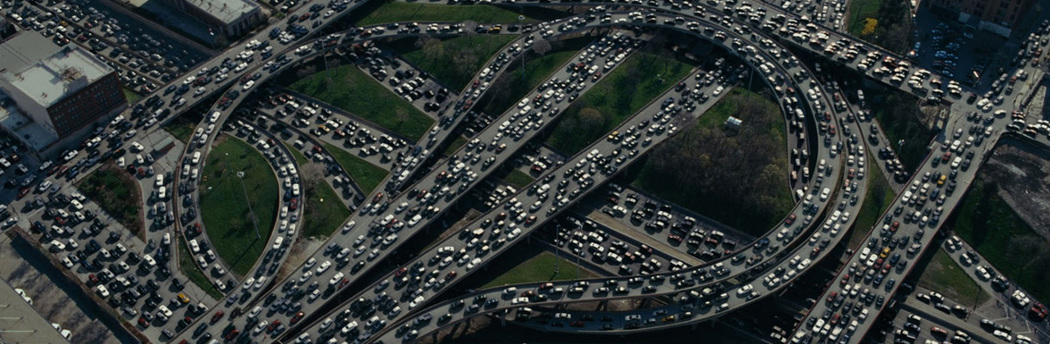
\includegraphics[keepaspectratio,width=0.75\textwidth]{images/deco1.jpg}
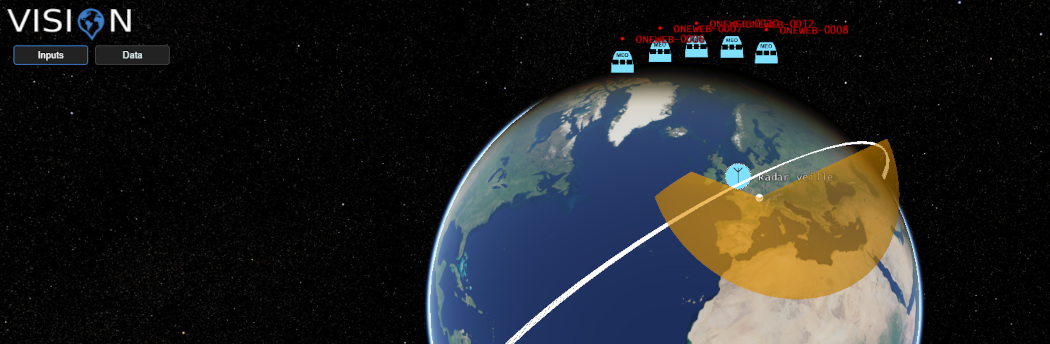
\includegraphics[keepaspectratio,width=0.75\textwidth]{images/deco2.jpg}
\end{center}

\end{frame}

\begin{frame}[noframenumbering]{Recall}
\begin{small}
\begin{itemize}
\item In Multi-Agent Systems, \textcolor{CS-1light}{the control is distributed}.\\
$\leadsto$ Each agent takes decision \textcolor{CS-1light}{autonomously}. 
\item Agents are situated in the same dynamic environment.\\ 
$\leadsto$ Possible \textcolor{CS-1light}{interactions} between agents' actions, and not always possible \textcolor{CS-1light}{to anticipate} this during the design of the system. 
\item Agents may share \textcolor{CS-1light}{limited resources}. 
\end{itemize}

\begin{center}
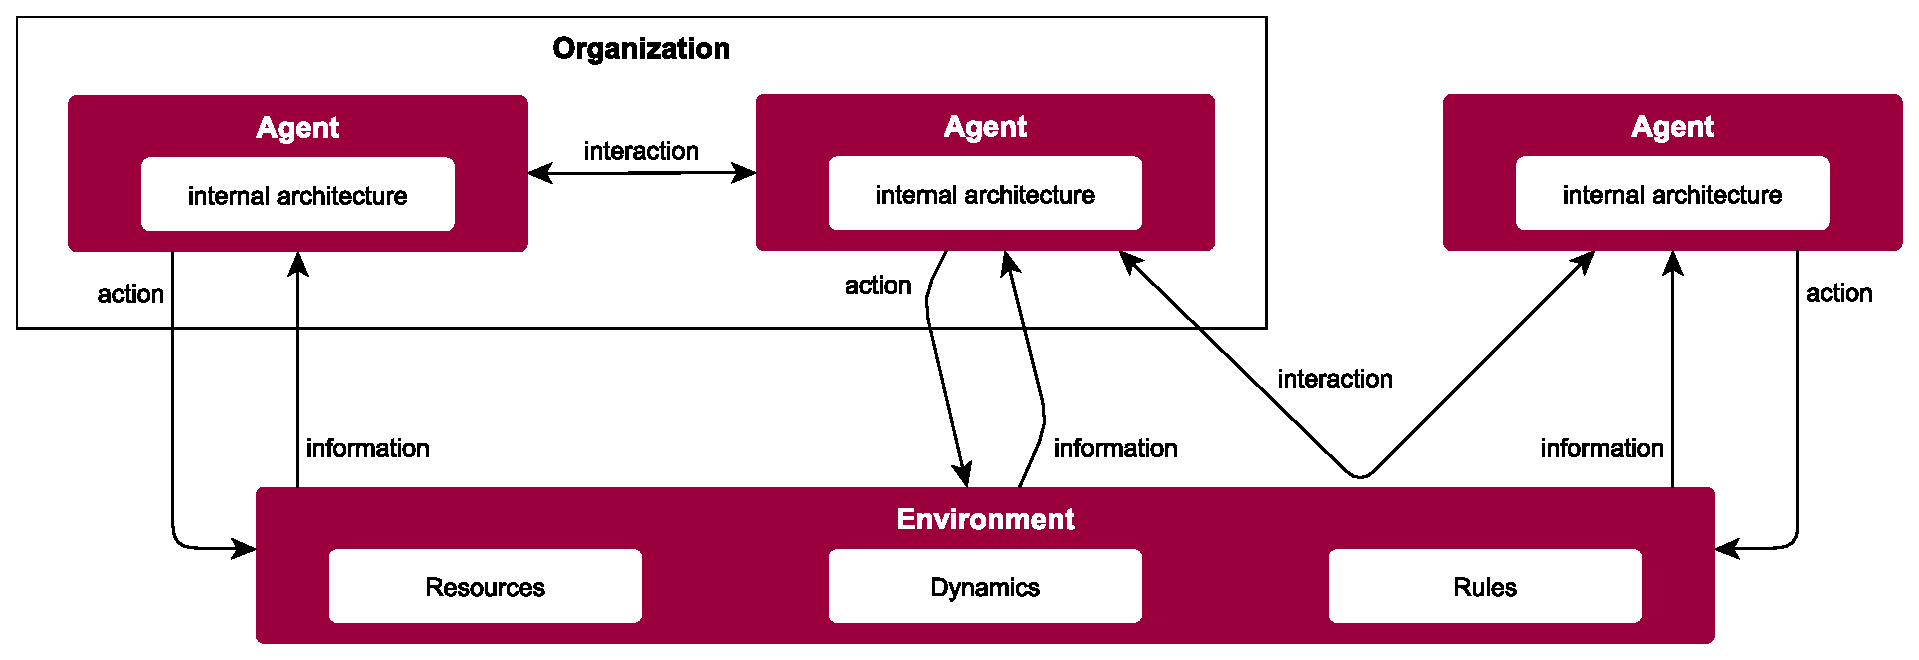
\includegraphics[keepaspectratio,width=0.95\textwidth]{images/mabs_details.eps}
\end{center}

\end{small}
\end{frame}

\begin{frame}[noframenumbering]{Coordination}
\begin{small}

Coordination is used in the case where individual agents actions can \textbf{interfere} with each other:
\begin{itemize}
\item \textcolor{CS-1light}{Positive interactions}: Share of actions, joint realization of actions, \dots
\item \textcolor{CS-1light}{Negative interactions}: Incompatibility of goals, access to limited resources, \dots
\end{itemize}

$\rightarrow$ Taking into account behavioral interactions allows to improve the behavior of agents: Resolution of issues, emergence of behaviors, etc. 

\end{small}
\end{frame}

\begin{frame}[noframenumbering]{Coordination}
\begin{small}

\textbf{Definition [Malon,1988]}
\begin{quotation}
"The set of supplementary activities which need to be carried out in a multi-agent environment, and which a single agent pursuing the same goals would not accomplish."  
\end{quotation}

\vspace{4mm}

\textbf{Definition [Ferber, 1995]}
\begin{quotation}
"The coordination of action can be defined as the articulation  of the individual actions accomplished by each agents in such a way that the whole ends up being a \textcolor{CS-1light}{coherent and high performance} operation. It is a matter of arranging the behaviors of the agents in time and space in such a way that the group action is improved, either through \textcolor{CS-1light}{better performance} or through \textcolor{CS-1light}{a reduction in conflict}. So the coordination of actions is one of the main methods of ensuring cooperation between autonomous agents." [Ferber, 1995] 
\end{quotation}

\end{small}
\end{frame}

\begin{frame}[noframenumbering]{Why coordination?}
\begin{small}

\begin{itemize}
\item The agents need \textcolor{CS-1light}{information and results} which only other agents can supply.\\
(\emph{e.g.} An agent supervising the activity of an industrial process at a given point will need information on the state of this process at other points).
\item The resources in the environment may be \textcolor{CS-1light}{limited}. Resources have to be shared in such a way as to optimise the actions to be carried out (\emph{e.g.} eliminating pointless actions, improving response times, reducing cost) while still trying to avoid any possible conflicts (\emph{e.g.} contradictory actions).
\item Optimize \textcolor{CS-1light}{costs} of actions (\emph{e.g.} eliminating pointless actions and avoiding redundant actions).
\end{itemize}

\end{small}
\end{frame}

\begin{frame}[noframenumbering]{Coordination mechanisms}
\begin{small}

\only<1>{
    \begin{center}
    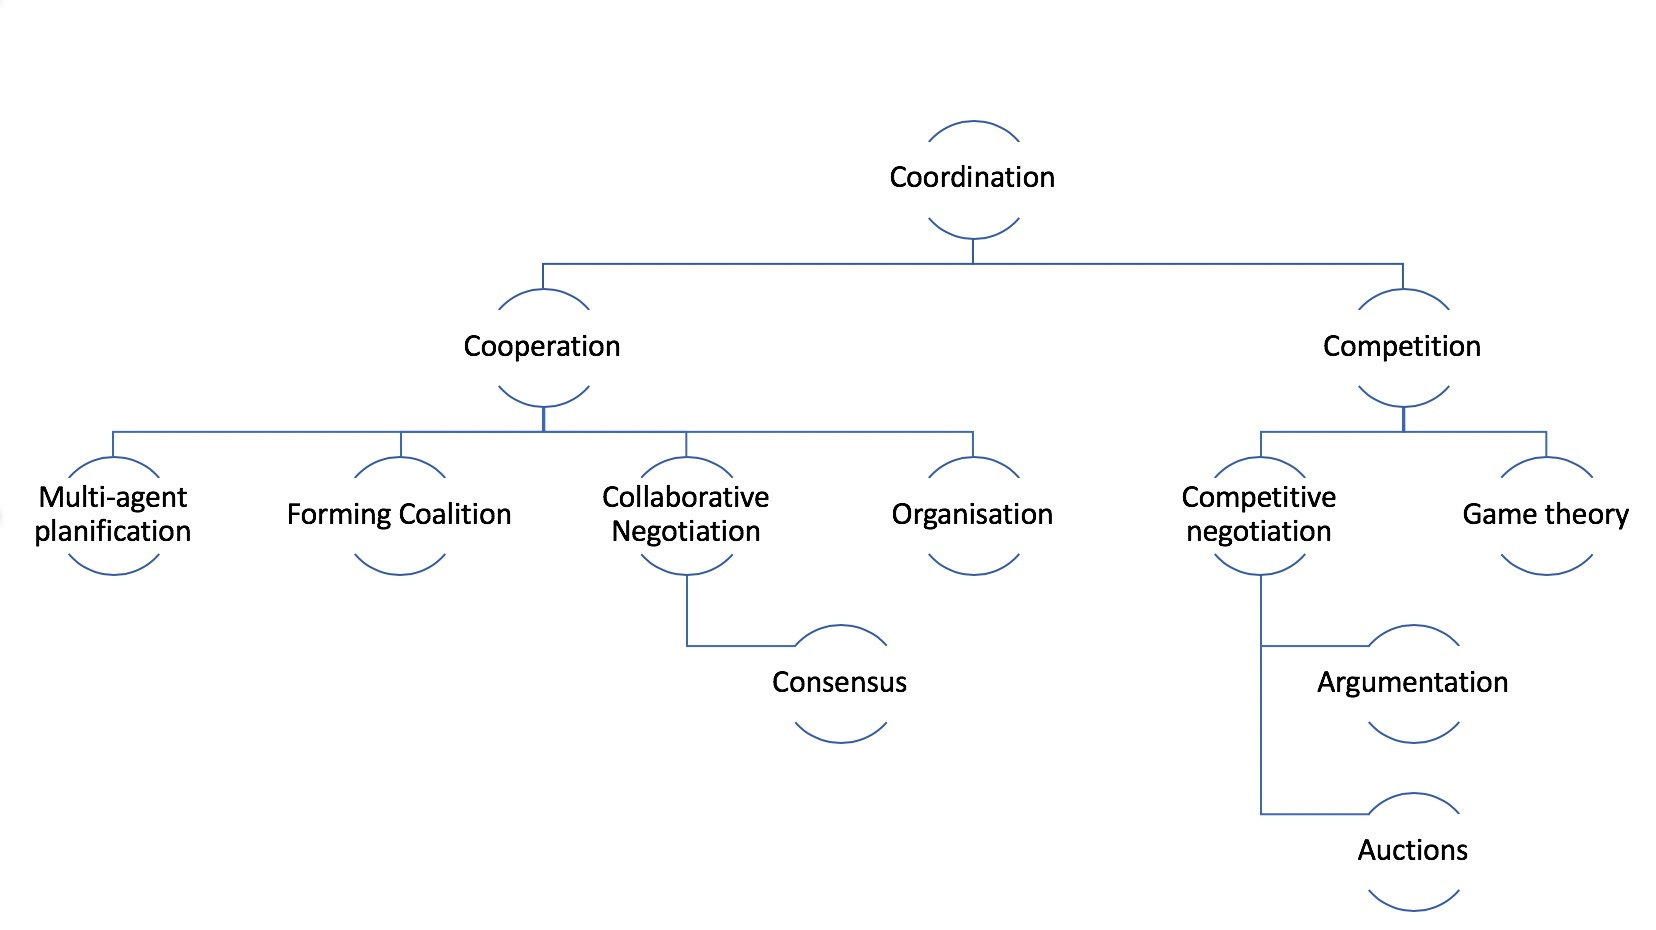
\includegraphics[keepaspectratio, width=1.00\textwidth]{images/coordination}\\
    {\footnotesize \emph{Source: Borrowed from Aurélie Beynier's course.}}
    \end{center}
}

\only<2>{
    \begin{center}
    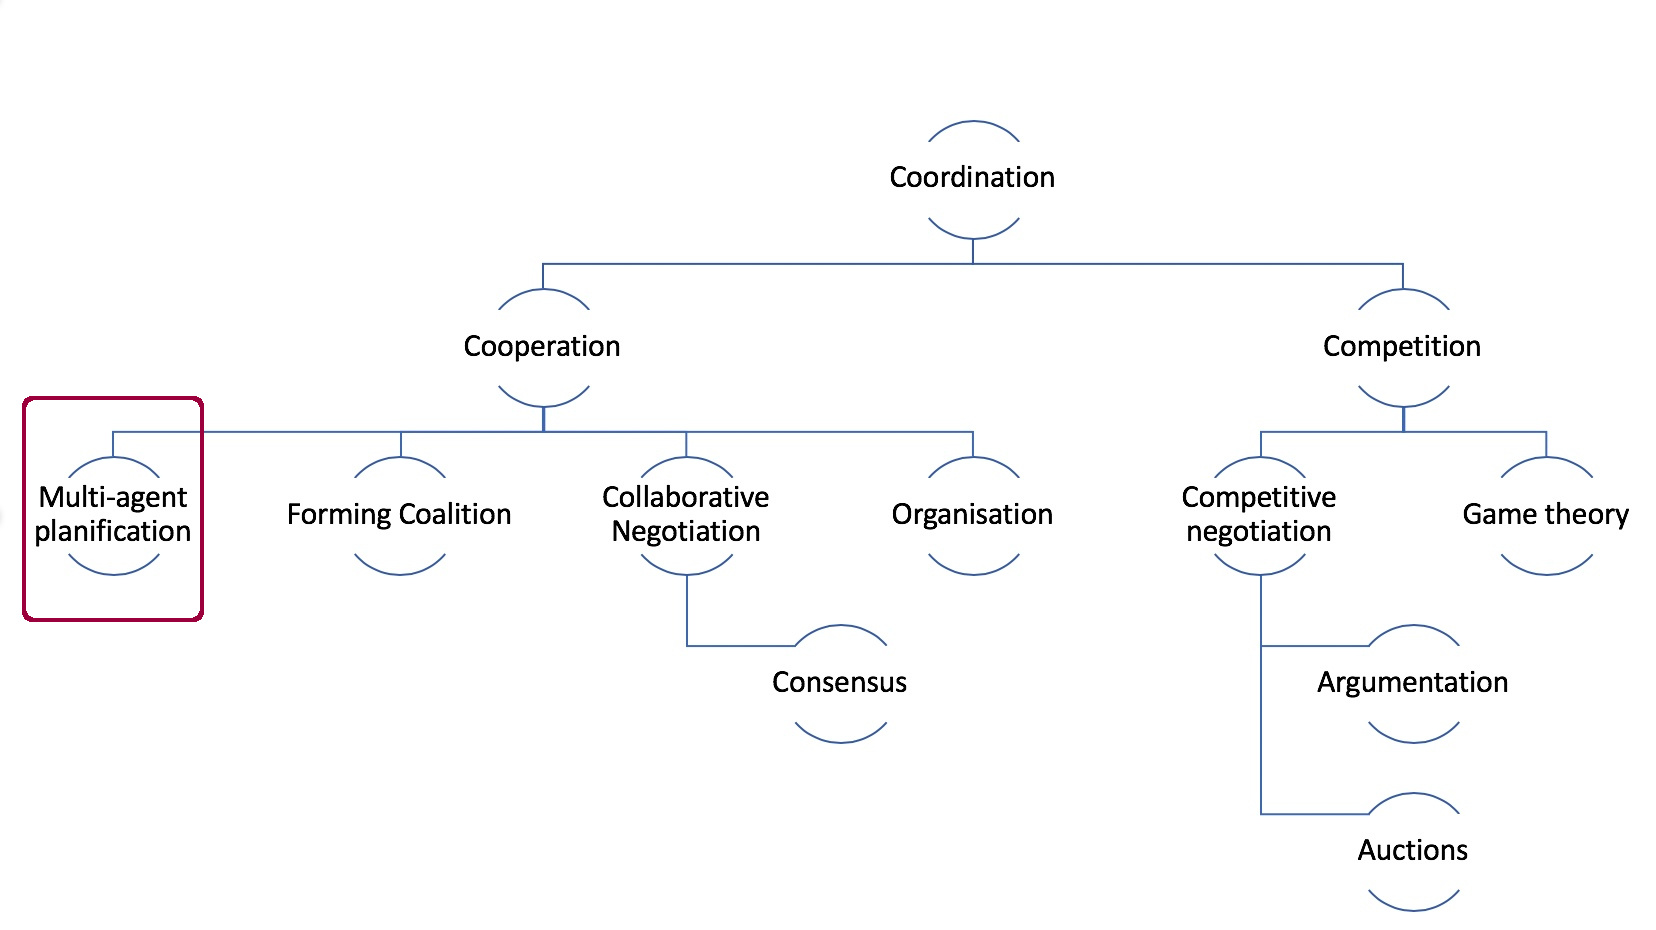
\includegraphics[keepaspectratio, width=1.00\textwidth]{images/coordinationselect}\\
    {\footnotesize \emph{Source: Borrowed from Aurélie Beynier's course.}}
    \end{center}
}

\end{small}
\end{frame}

% Table of contents
\begin{frame}[noframenumbering]{Table of contents}
	\textcolor{CS-2}{\textbullet \hskip5pt \textbf{First Intuition on Planning}}\\
	\begin{small}
		\emph{What is Planning? Concepts, motivations, objectives.}\\
	\end{small}
	
	\vspace{4mm}
	
	\textcolor{CS-2}{\textbullet \hskip5pt \textbf{Multi-Agent Planning}}\\
	\begin{small}
		\emph{Why and how use planning in Multi-Agent Systems?}\\
	\end{small}
	
	\vspace{4mm}
	
	\textcolor{CS-2}{\textbullet \hskip5pt \textbf{Automated Planning}}\\
	\begin{small}
	    \emph{How automated planning works?}\\
	\end{small}
	
	\vspace{4mm}
	
	\textcolor{CS-2}{\textbullet \hskip5pt \textbf{Solving Automated Planning Problems}}\\
	\begin{small}
	    \emph{How to solve automated planning problems?}\\
	\end{small}
	
	\vspace{4mm}
	
	\textcolor{CS-2}{\textbullet \hskip5pt \textbf{Practical Works}}\\
	\begin{small}
	    \emph{}
	\end{small}
	
\end{frame}
\endgroup


\section{First Intuition on Planning}

\begin{frame}{Intuitive Planning Definition}
\begin{small}

\textbf{What is Planning?}\\
\begin{itemize}
\item Planning is the \textcolor{CS-1light}{reasoning side of acting}. It is an abstract, explicit deliberation process that chooses and organizes actions by anticipating their outcomes.
\item This deliberation aims at achieving \textcolor{CS-1light}{as best as possible} some objectives.
\item Automated planning is an area of Artificial Intelligence (AI) that studies this deliberation process computationally.
\end{itemize}

\textbf{Book:} \emph{M. Ghallab, D. Nau and P. Traverso Automated Planning Theory and Practice Morgan Kaufmann, 2004}

\end{small}
\end{frame}

\begin{frame}{Practical agent (recall from Basic Course)}
\begin{small}

\textbf{Means-ends reasoning/planning}\\
\begin{itemize}
\item Planning is the design of a course of actions that will achieve some desired goal.
\item Planning system required:
\begin{itemize}
\item (representation of) goal/intention to achieve,
\item (representation of) actions it can perform,
\item (representation of) the environment.
\end{itemize}
\item Planning system generates a plan to achieve the goal.
\end{itemize}

\begin{center}
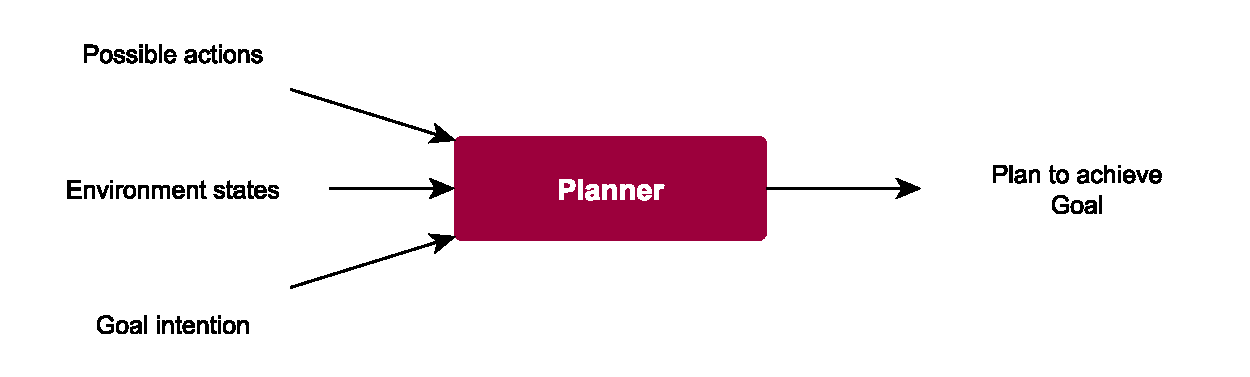
\includegraphics[keepaspectratio, width=0.75\textwidth]{images/planning.eps}
\end{center}
\end{small}
\end{frame}

\begin{frame}{Automated Planning Motivations}
\begin{small}

\begin{itemize}
\item \textcolor{CS-1light}{Practical Motivations}: Designing information processing tools that give access to affordable and efficient planning resources.
\item \textcolor{CS-1light}{Theoretical Motivations}: Planning is an important component of
rational behaviour.
\end{itemize}

\pause

\begin{exampleblock}{Rescue operation after a natural disaster!}
\begin{itemize}
\item It involves a large number of actors and requires transportation infrastructures.
\item It relies on careful planning and assessment of several alternate plans.
\item It is time constrained and demands immediate decisions that must be supported with a planning tool.
\end{itemize}
\end{exampleblock}

\end{small}
\end{frame}

\begin{frame}{Planning}
\begin{small}

\begin{itemize}
\item Necessary when \textcolor{CS-1light}{near-term} choices of actions can enable, or prevent, later action choices required to achieve goals.
\item Possible when agent possesses a \textcolor{CS-1light}{sufficiently detailed and correct model} of the environment, and how action affect the environment.
\item Challenging because the space of possible plans \textcolor{CS-1light}{grows exponentially} with the plan duration.
\end{itemize}

\end{small}
\end{frame}

\begin{frame}{Conceptual Model of Planning}
\begin{small}

\textbf{State Transition System:}\\
The conceptual model of planning can be represented as a state transition system. Formally, it is a 4-tuple $\Sigma=(S,A,E,\gamma)$:

\begin{itemize}
\item $S=\{s_0, s_1, \dots, s_n\}$ is a finite set of states\\(\textit{the possible states the world can be in}),
\item $A= \{a_0, a_1, \dots, a_n\}$ is a finite set of actions\\(\textit{the actions that can be performed by some agent in the world}),
\item $E=\{e_0, e_1, \dots, e_n\}$ is a finite set of events\\(\textit{the events that can occur in the world}),
\item $\gamma: S \times A \times E \rightarrow 2^S$ is a state transition function\\(\textit{the function describing how the world evolves when actions and events occur}).
\end{itemize}

A state transition system may be represented by a directed graph whose nodes are the state is $S$.

\textbf{Note:} \emph{$2^S$ means powerset of $S$, maps to a set of states}.

\end{small}
\end{frame}

\begin{frame}{Planning Objectives}
\begin{small}

Given a state transition $\Sigma$, the purpose planning is to find \textcolor{CS-1light}{which actions} to apply to \textcolor{CS-1light}{which states} in order to achieve \textcolor{CS-1light}{some objective} when starting from a given situation. A plan is a structure that gives the appropriate actions. \textcolor{CS-1light}{The objective}  can be expressed : 
\begin{enumerate}
\item By simply specifying a \textcolor{CS-1light}{goals state} $s_g$ or a set of goal states $S_g$. In this case, the objective is achieved by any sequence of state transition that ends at one of the goal states.
\item By \textcolor{CS-1light}{the satisfaction of some conditions} over the sequence of state followed by the system.
\item By \textcolor{CS-1light}{a utility function} attached to \textcolor{CS-1light}{each state}, with \textcolor{CS-1light}{penalties and rewards}. The goal is to optimize some compounded function of these utilities.
\item As \textcolor{CS-1light}{tasks} that the system should perform.
\end{enumerate}

\end{small}
\end{frame}

\begin{frame}{Graphical Representation of Planning Model}
\begin{small}

It is convenient to depict conceptual planning model through the interaction between three components:
\begin{itemize}
\item A \textcolor{CS-1light}{state transition system} $\Sigma$ evolves as specified by its state transition function $\gamma$ according to the events and actions that it receives.
\item  A \textcolor{CS-1light}{controller,} given as input the state $s$ of the system, provides as output an action $a$ according to some plan.
\item A \textcolor{CS-1light}{planner}, given as input a description of the system $\Sigma$, an initial situation, and some objective, synthesizes a plan for the controller in order to achieve the objectives.
\end{itemize}

\begin{center}
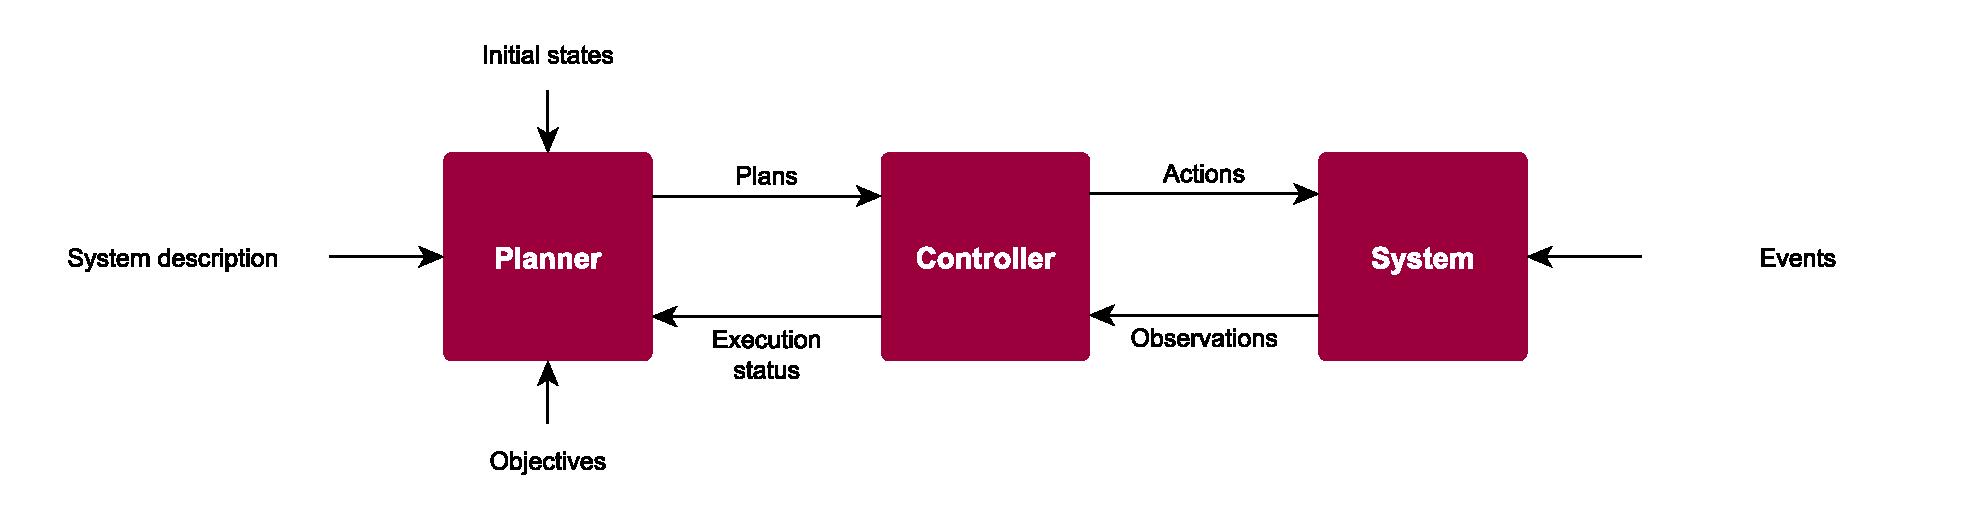
\includegraphics[keepaspectratio, width=0.90\textwidth]{images/planning_model.eps}\\
{\footnotesize \emph{Source: Borrowed from Damien Pellier's course.}}
\end{center}
\end{small}
\end{frame}

\section{Multi-Agent Planning}

\begin{frame}{Multi-Agent Planning}
\begin{small}
\begin{itemize}
\item Multi-Agent Planning (MAP) introduces a new perspective in the resolution of a planning task with the \textcolor{CS-1light}{adoption of a distributed problem-solving scheme} instead of the classical single-agent planning paradigm.
\item Distributed planning is required \emph{"when planning knowledge or responsibility is distributed among agents or when the execution capabilities that must be employed to successfully achieve objectives are inherently distributed"} [desJardins et al. 1999].
\end{itemize}

\textbf{Article:} \emph{Weerdt, Mathijs \& Clement, Bradley. (2009). Introduction to planning in multiagent systems. Multiagent and Grid Systems. 5. 345-355. 10.3233/MGS-2009-0133.}
\end{small}
\end{frame}

\begin{frame}{Multi-Agent Planning}
\begin{small}

\textbf{What is a plan?}\\
A (partially) ordered sequence of actions such that the execution makes it possible to achieve the desired goals or to maximize a performance measure.

\begin{alertblock}{Challenges}
\begin{itemize}
\item  The actions of an agent have a more or less long-term consequences on the \textcolor{CS-1light}{other} agents (actions, objectives).
\item It is not effective for agents to plan \textcolor{CS-1light}{independently} of one another.
\item Challenging because the space of possible plans grows exponentially with the plan duration, and of multi-agent plans grows exponentially in the \textcolor{CS-1light}{number of agents}.
\item \textcolor{CS-1light}{Coordination} required between agents (whether they are cooperatives or competitive).
\end{itemize}
\end{alertblock}

\end{small}
\end{frame}

\begin{frame}{Multi-Agent Planning Modes}
\begin{small}

Planning actions in MAS universes can be broken down into three distinct stages: making plans, synchronizing/coordinating plans, and executing plans. 

\begin{center}
\begin{figure}
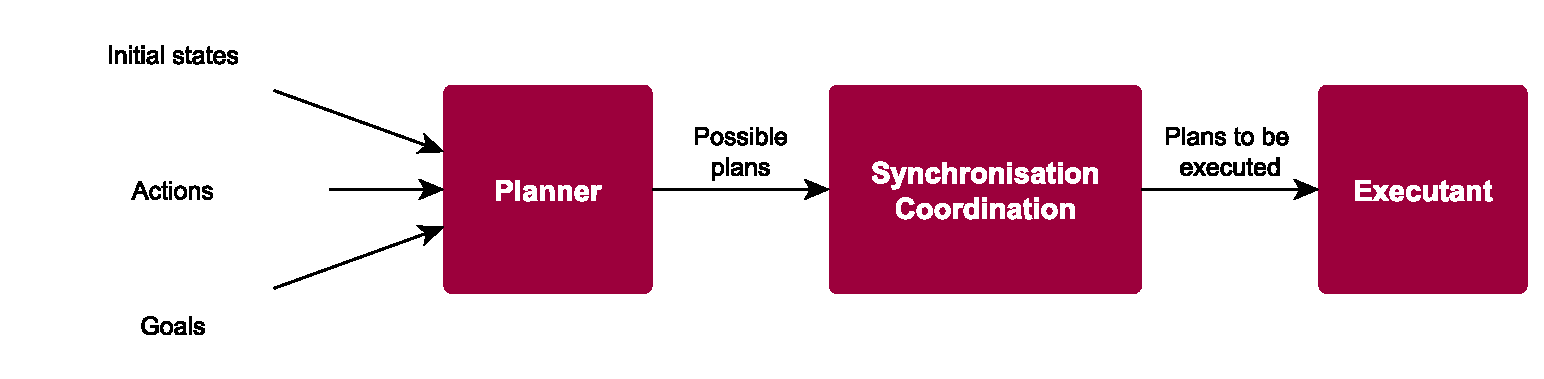
\includegraphics[keepaspectratio, width=0.95\textwidth]{images/mas_planning.eps}
\end{figure}
\end{center}

\textbf{Different modes:}
\begin{itemize}
\item Centralized \textcolor{CS-1light}{Planning} for multiple agents.
\item Centralized \textcolor{CS-1light}{Coordination} for partial Plans.
\item \textcolor{CS-1light}{Distributed} planning.
\end{itemize}

\end{small}
\end{frame}

\begin{frame}{Centralized planning for multiple agents}
\begin{small}
\begin{itemize}
\item Assumes that only \textcolor{CS-1light}{a single planner} exists (a single agent capable of planning and organizing actions for all agents).
\item Handles the synchronizing of plans together with the allocation of tasks to the other agents (executants).
\item Assumes that the planner has an \textcolor{CS-1light}{exact knowledge of the environment} and is able  to anticipate its evolution.
\item The agents (executants) should send their \textcolor{CS-1light}{private} knowledge to the planner (preferences for instance).
\end{itemize}

\begin{center}
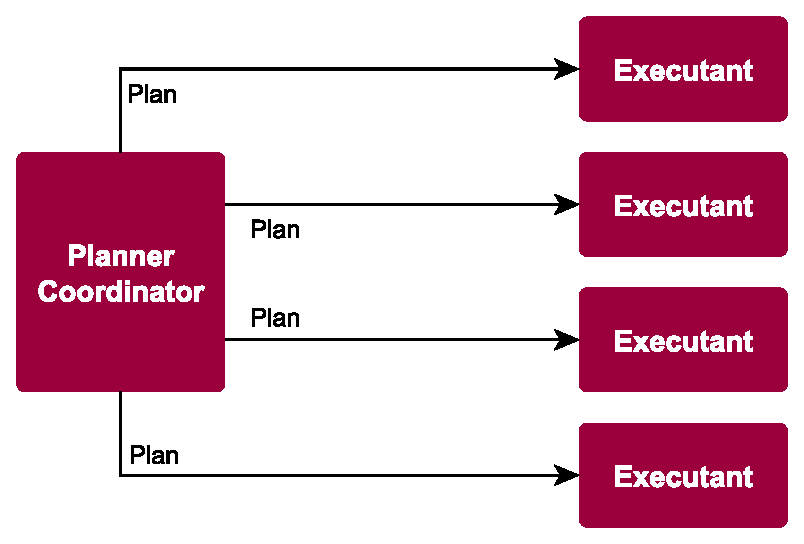
\includegraphics[keepaspectratio, width=0.45\textwidth]{images/mas_planning_centralized.eps}
\end{center}
\end{small}
\end{frame}


\begin{frame}{Centralized planning for multiple agents}
\begin{small}
\textbf{Three stages:}
\begin{enumerate}
\item The first step is to look for a general plan, which can be expressed in the form of a cyclic diagram.
\item We then determine the branches which can be executed in parallel, and we introduce synchronisation points each time two computation branches join together.
\item Finally, we allocate the execution of the tasks to the various agents concerned.
\end{enumerate}
\end{small}
\end{frame}


\begin{frame}{Centralized planning for multiple agents}
\begin{small}
\begin{exampleblock}{Example: Two robots manipulating the cubes}
\begin{center}
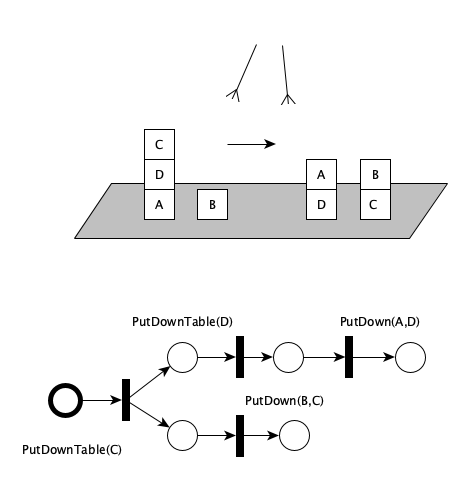
\includegraphics[scale=0.35]{images/central_planning}
\end{center}
\end{exampleblock}
\end{small}
\end{frame}

\begin{frame}{Distributed planning}
\begin{small}
\begin{itemize}
\item \textcolor{CS-1light}{No centralizing} agent either for drawing up overall plans or coordinating partial plans. 
\item \textcolor{CS-1light}{Each agent individually plans} the actions it intends to carry out, depending of its own goal. 
\itemNo Difficulties: Resolution of potential conflicts, recognition of the synergetic situations
%which can occure when the actions of one group may be useful for achieving the goals of others, so that thez agents are of service to each other. 
\end{itemize}

\vspace{4mm}

\begin{center}
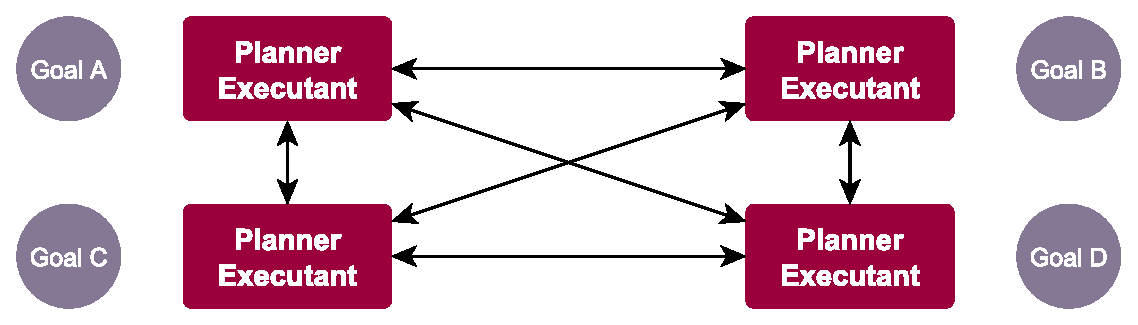
\includegraphics[keepaspectratio, width=0.75\textwidth]{images/mas_planning_distributed.eps}\\
{\footnotesize The problem of the agents consists of exchanging information relating to their plans and their goals, so that each of them may achieve its objectives.} 
\end{center}
\end{small}
\end{frame}

\begin{frame}{Distributed planning}
\begin{small}
\begin{itemize}
\item \textcolor{CS-1light}{Cooperative Distributed Planning (CDP)}: Focuses on \textbf{planning} and how it can be extended into a distributed environment, where the process of formulating or executing a plan could involve a number of participants. 
\item \textcolor{CS-1light}{Negotiated distributed planning (NDP)}: Focuses on \textbf{coordinating and controlling the actions} of multiple agents in a shared environment, and has adopted planning representations and algorithms as a mean to do that end. 
\end{itemize}
\end{small}
\end{frame}

\begin{frame}{Cooperative Distributed Planning: Common questions.}
\begin{small}
\begin{itemize}
\item How the plans or partial plans are represented? 
\item What are the methods for generating the plans?
\item How the tasks are allocated to agents? 
\item How the agents communicate with each other during the planning? 
\item How the agents coordinate their actions?
\end{itemize}

\vspace{4mm}

$\leadsto$ \textbf{\textcolor{CS-1light}{Centralized coordination}} of distributed plans.\\

$\leadsto$ \textbf{\textcolor{CS-1light}{Distributed coordination}} of distributed plans.
\end{small}
\end{frame}

\begin{frame}{CDP: Centralized coordination of distributed plans}
\begin{small}

\begin{itemize}
\item Each agent independently draws up it own partial plan, which is sends to the coordinator. 
\item The coordinator synthesize all the partial plans into a single coherent overall plan. 
\item The coordinator communicates to synchronize the agents actions. 
\item Objectives: Avoid conflicts and parallelize actions as much as possible.
\begin{itemize}
\item Identification of unsafe (conflicting) situations.
\item Insertion of synchronization primitives to avoid such situations. 
\end{itemize}
\end{itemize}

\begin{center}
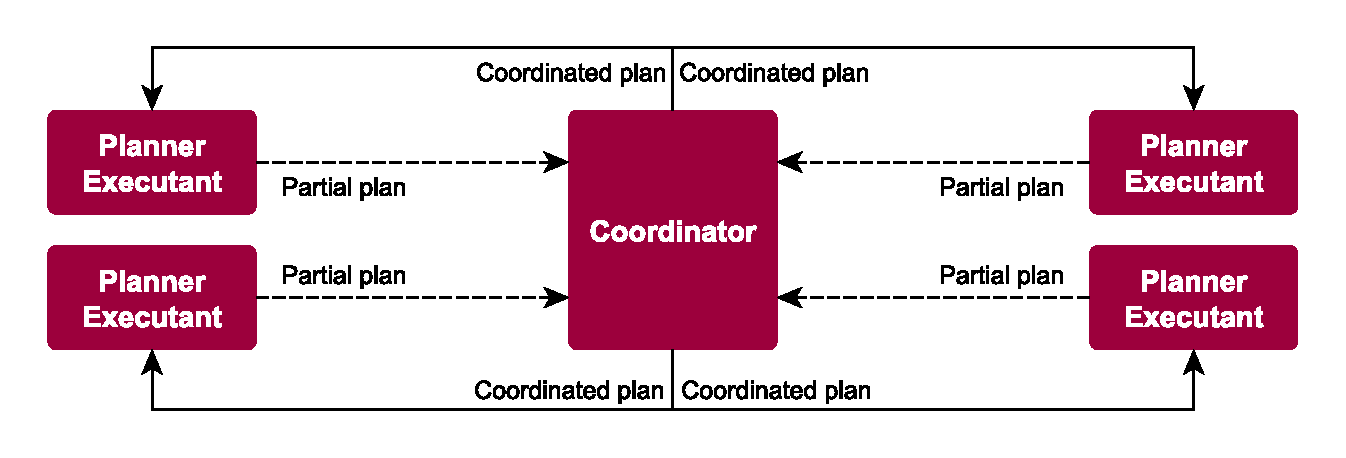
\includegraphics[keepaspectratio,width=0.75\textwidth]{images/mas_planning_cdp_central.eps}
\end{center}
\end{small}
\end{frame}

\begin{frame}{CDP: Centralized coordination of distributed plans}
\begin{small}

\begin{alertblock}{Limits}
\begin{itemize}
\item Uncontrollable system in case of faulty coordinator.
\item Bottleneck at coordinator level.
\item Very high communication load: communications with the coordinator as soon as you reach a critical area.
\item Loss of data confidentiality.
\item Question of the neutrality of the central coordinator.
\end{itemize}
\end{alertblock}

\end{small}
\end{frame}

\begin{frame}{CDP: Distributed coordination of distributed plans}
\begin{small}

\begin{itemize}
\item Reduce the communication.
\item Allows parallel resolution of coordination.
\item Greater robustness.
\item Possibility of keeping confidential data (privacy).
\end{itemize}

\pause

\vspace{4mm}

\textbf{Partial Global Planning [Durfee, 1988]:}\\
Framework for the coordination of distributed systems in a dynamic and non predictable environment: 
\vspace{-2mm}
\begin{itemize}
\item Agents continually re-plan.
\item Changes in an agent's plan influence others agents who replan in turn. 
\item Planning is continuous and agents need to revise and continue their plans despite the fact that they can be temporarily non-coordinated.
\end{itemize}

\end{small}
\end{frame}

\begin{frame}{CDP: Distributed coordination of distributed plans}
\begin{small}

\textbf{Partial Global Planning [Durfee, 1988]:}\\
Cooperating agents \textcolor{CS-1light}{exchange information} in order to reach common conclusion about the problem-solving process.
\vspace{-2mm}
\begin{itemize}
\item \textcolor{CS-1light}{Partial}: The system does not (indeed cannot) generate a plan for the entire problem.
\item \textcolor{CS-1light}{Global}: Agents form non-local plans by exchanging local plans and cooperating to achieve a non-local view of problem solving.  
\end{itemize}

\vspace{4mm}

Three iterated stages:
\vspace{-2mm}
\begin{enumerate}
\item \textcolor{CS-1light}{Each agent} decides what its own goals are and \textcolor{CS-1light}{generates short-term plans} in order to achieve them.
\item Agents \textcolor{CS-1light}{exchange information} to determine where plans and goals interact.
\item Agent \textcolor{CS-1light}{alter local plan} in order to better coordinate their own activities.
\end{enumerate}

\end{small}
\end{frame}

\begin{frame}{CDP: Distributed coordination of distributed plans}
\begin{small}

\begin{itemize}
\item \textcolor{CS-1light}{Communication}: To prevent incoherence $\leadsto$ \textcolor{CS-1light}{Meta-level structure} to guide the cooperation.
\item It indicates which agents an agent should exchange information with, and under what conditions they should do. 
\item Actions and interactions of a group of agents are incorporated into a data structure: \textcolor{CS-1light}{partial Global plan (PGP)}:
\begin{itemize}
\item \textcolor{CS-1light}{Objective}: The larger goal that the system is working towards.
\item \textcolor{CS-1light}{Activity maps}: Representation of what agents are actually doing, and what results will be generated by their activities.
\item \textcolor{CS-1light}{Solution construction graph}: Representation of how agents should interact, and what information should be exchanged, and when, in order for the system to successfully generate a result.
\end{itemize}
\end{itemize}

\end{small}
\end{frame}

\begin{frame}{Negotiation Distributed Planning}
\begin{small}

\textbf{Coordination through Join Intentions:} Using the notion of "\textcolor{CS-1light}{human teamwork models}".

\begin{itemize}
\item The agents have a team model: Goals and plans of the team.
\item Teams members may communicate to attain mutual beliefs while building joint intentions. 
\item Ease monitoring of team performance and recognition of special situations (e.g. failure), very useful in dynamic environments.
\end{itemize}

\end{small}
\end{frame}

\begin{frame}{NDP: Join Intention Theory}
\begin{small}

\begin{itemize}
\item  A team $\theta$ jointly intends a team action if team members are jointly committed to completing that team actions.
\item A \textcolor{CS-1light}{joint persistent goal (JPG)}: A joint commitment to achieve $p$ (completion of a team action) is denoted, $JPG(\theta, p,q)$. $q$ is an irrelevance clause $\leadsto$ t enables a team to drop the JPG should they mutually believe $q$ to be false.
\item Three conditions:
\begin{enumerate}
\small 
\item All team members mutually believe that $p$ is currently false.
\item All team members have $p$ as their mutual goal (they want $p$ to be eventually true).
\item All teal members believe that until $p$ is mutually known to be achieved, unachievable or irrelevant they mutually believe that they each hold $p$ as a weak achievement goal: $WAG(\mu,p, \theta, q )$ ($\mu $: a team member).
\end{enumerate}
\item The commitment to attain mutual belief in the termination of $p$ is a key aspect of a $JPG$.
\end{itemize}

\end{small}
\end{frame}

\begin{frame}{NDP: Coordination through Join Intentions}
\begin{small}

\begin{exampleblock}{Example: Coordinated attack of a fleet of helicopters}
\begin{center}
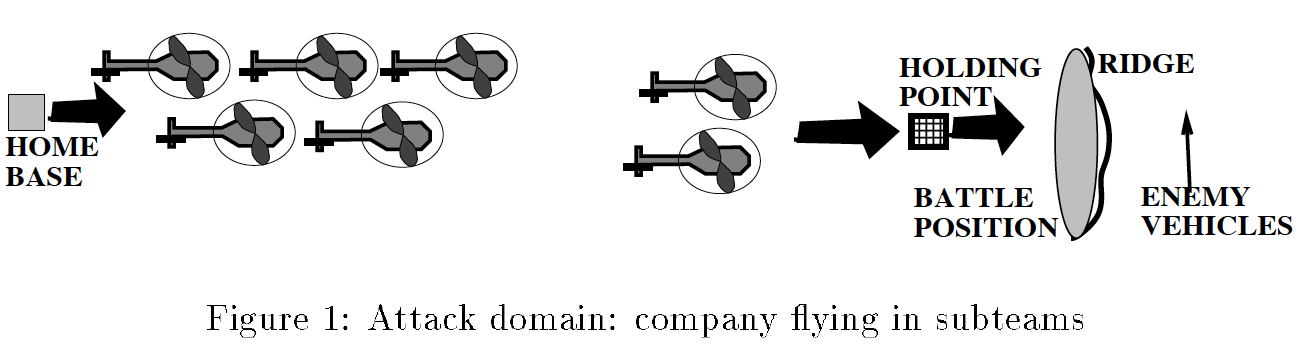
\includegraphics[keepaspectratio,width=0.75\textwidth]{images/STEAM.png}
\end{center}

\begin{itemize}
\item Pilot agents for a company of (up to eight) synthetic attack helicopters.
\item The company starts at the home-base, where the commander pilot agent first sends orders and instructions to the company members.
\item The company processes these orders and then begins flying towards their specified battle position, i.e., the area from which the company will attack the enemy.
\item While on the way to the battle position, depending on the orders, the company members may fly together or dynamically split into pre-determined subteams.
\end{itemize}
\end{exampleblock}

\end{small}
\end{frame}

\begin{frame}{Going further !!}
\begin{small}

$\rightarrow$ \textbf{Planning under uncertainty} [Russel and Norvig, 2003]

\begin{itemize}
\item Markov Decision Processes (MDP)
\item Partially Observable Markov Decision Processes (POMDP)
\item Decentralized Partially Observable Markov Decision Processes (DEC-POMDP)
\item ...
\end{itemize}
\end{small}
\end{frame}

\section{Automated Planning}


\begin{frame}{Path and Motion Planning}
\begin{small}

\textcolor{CS-1light}{\textbf{Path and Motion Planning}} is concerned with the synthesis of a geometric path from a starting position in space to a goal and a control trajectory along that path that specifies the state variables in the configuration space of mobile systems, such as a truck, a mechanical arm, a robot,etc.

Motion planning takes into account:
\begin{itemize}
\item The model of the environment;
\item The kinematic constraints;
\item The dynamic constraints.
\end{itemize}
\end{small}
\end{frame}

\begin{frame}{Perception Planning}
\begin{small}
\textcolor{CS-1light}{\textbf{Perception Planning}} is concerned with plans involving sensing actions forgathering informations. It arises in tasks such as modelling environments or objects, identifying objects, localizing through sensing a mobile system, or more generally identifying the current state of the environment.

\begin{itemize}
\item Perception planning addresses question such as information needed and when it is needed, where to look for it, which sensors are most adequate for a particular task and how to use them.

\item It relies on decision theory for problems of which and when information is needed, on mathematical programming and constraint satisfaction for viewpoint selection and the sensor modalities.
\end{itemize}
\end{small}
\end{frame}

\begin{frame}{Navigation Planning}
\begin{small}
\textcolor{CS-1light}{\textbf{Navigation Planning}} combines the two previous problems of motion and perception planning in order to reach a goal or to explore an area. The purpose of navigation planning is to synthesize a policy that combines localization primitives and sensor-based motion primitives.
\end{small}
\end{frame}

\begin{frame}{Manipulation Planning}
\begin{small}
\textcolor{CS-1light}{\textbf{Manipulation Planning}} is concerned with handling objects, e.g. to build assemblies. It arises in dialog and in cooperation problems between several agents, human or artificial. It addresses issues such as when and how to query needed information and which feedback should be provided.

\begin{itemize}
\item The actions include sensory information.
\item A plan might involve picking up an object from its marked sides, returning it if needed, inserting it into an assembly, and pushing lightly till it clips mechanically into position.
\end{itemize}
\end{small}
\end{frame}

\begin{frame}{Domain Specific Approaches}
\begin{small}
\textbf{Domain specific approaches} to specific forms of planning are certainly well justified. However, they are frustrating for several reasons.

\begin{enumerate}
\item Some commonalities to all these forms of planning are not addressed in the domain specific approaches. The study of these commonalities is needed for understanding the process of planning.
\item It is more costly to address each planning problem anew instead of relying on and adapting some general tools.
\item Domain specific approaches are not satisfactory for studying and designing an autonomous intelligent machine. Its deliberative capabilities will be limited to areas for which it has a domain specific planner.
\end{enumerate}
\end{small}
\end{frame}

\begin{frame}{Domain Independent Approaches}
\begin{small}
\textbf{Domain independent approaches} relies on abstract, general models of actions.These models range from simple ones that allow only for limited forms of reasoning to models with richer prediction capabilities. There are in particular the following forms of models and planning capabilities.

\begin{enumerate}
\item Project Planning in which models of actions are reduced mainly to temporal and precedence constraints, e.g. the earliest and the latest start times of an action or its latency with respect to another action. Project planning is used for interactive plan edition and verification.
\item Scheduling and resources allocation in which the action models include the above types of constraints plus constraints on the resources to be used by each action.
\item Plan synthesis in which the action models enrich the precedent models with the conditions needed for applicability of an action and the effects of the action on the state of the world.
\end{enumerate}
\end{small}
\end{frame}

\begin{frame}{Conceptual Model of Planning}
\begin{small}

\textbf{State Transition System:}\\
The conceptual model of planning can be represented as a state transition system. Formally, it is a 4-tuple $\Sigma=(S,A,E,\gamma)$:

\begin{itemize}
\item $S=\{s_0, s_1, \dots, s_n\}$ is a finite set of states\\(the possible states the world can be in),
\item $A= \{a_0, a_1, \dots, a_n\}$ is a finite set of actions\\(the actions that can be performed by some agent in the world),
\item $E=\{e_0, e_1, \dots, e_n\}$ is a finite set of events\\(the events that can occur in the world),
\item $\gamma: S \times A \times E \rightarrow 2^S$ is a state transition function\\(the function describing how the world evolves when actions and events occur).
\end{itemize}

A state transition system may be represented by a directed graph whose nodes are the state is $S$.

\textbf{Note:} \emph{$2^S$ means powerset of $S$, maps to a set of states}.

\end{small}
\end{frame}

\begin{frame}{Crane and robot transportation example}
\begin{small}

\begin{center}
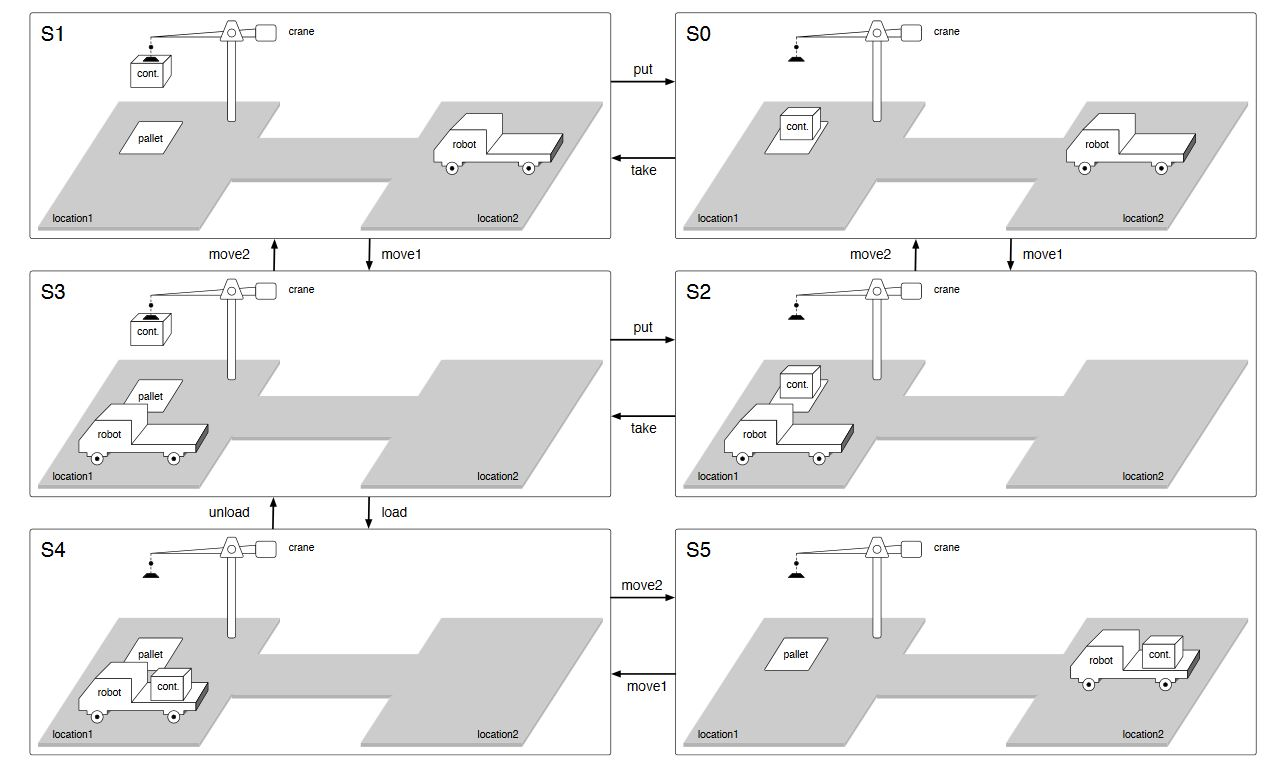
\includegraphics[keepaspectratio, width=0.90\textwidth]{images/automated_planning_example1.jpg}
\end{center}

\vspace{-4mm}

Crane and robot transportation example shows a state transition system involving a container in a pile, a crane that pick up and put down the container and a robot that can carry the container and move it from one location to another.
\end{small}
\end{frame}

\begin{frame}{Crane and robot transportation example}
\begin{small}

In this example:
\begin{itemize}
\item The set of states is $S=\{s_0, s_1, s_2, s_3, s_4, s_5\}$
\item The set of actions is $A=\{take, put, load, unload, move1, move2\}$
\item The set of events $E$ is empty
\item the transition function $\gamma$ is defined by : if $a$ is an action and $\gamma(s,a)$ is not empty then $a$ is applicable to state $s$.
\end{itemize}

\end{small}
\end{frame}

\begin{frame}{Restricted Model}
\begin{small}

Planning model puts forward various restrictive assumptions, particularly the following ones.
\begin{itemize}
\item \textbf{Finite $\Sigma$.} The system $\Sigma$ has a finite set of states.
\item \textbf{Fully Observable $\Sigma$.} The system $\Sigma$ is fully observable, i.e. one has complete knowledge about the state of $\Sigma$.
\item \textbf{Deterministic $\Sigma$.} The system $\Sigma$ is deterministic, i.e. for every states $s$ and for every event of action $u$, if an action is applicable to a state, its application brings a deterministic system to a single other state.
\item \textbf{Static $\Sigma$.} The system $\Sigma$ is static, i.e. the set of event $E$ is empty. $\Sigma$ has no internal dynamics.
\end{itemize}

\end{small}
\end{frame}

\begin{frame}{Restricted Model}
\begin{small}

\begin{itemize}
\item \textbf{Restricted Goals.} The planner handles only restricted goals that a respecified as an explicit goal state $s_g$ or a set of goal states $S_g$.
\item \textbf{Sequential Plans.} A solution plan to a planning problem is a linearly ordered finite sequence of actions.
\item \textbf{Implicit time.} Actions and events have no duration. They are instantaneous, state transitions. This assumptions is embedded in state transition systems, a model that does not represent time explicitly.
\item \textbf{Offline Planning.} The planner is not concerned with any change that may occur in $\Sigma$ while it is planning. It plans for a given initial and goal states regardless of the current dynamics, if any.
\end{itemize}
\end{small}
\end{frame}

\begin{frame}{Classical Representation for Planning}
\begin{small}

There are three different ways to represent classical planning problems. Each of them is equivalent in expressive power.

\begin{itemize}
\item \textbf{Set theoric representation.} Each state of the world is a set of propositions and each action is a syntactic expression specifying which propositions belong to the state in order for the action to be applicable and which propositions the action will add or remove to change the state of the world.
\item \textbf{Classical representation.} The states and the actions are like the ones described for set theoric representation except that first order literals and logical connectives are used instead propositions.
\item \textbf{State variable representation.} Each state is represented by a tuple of value $n$ state variables $\{x_1, \dots, x_n\}$ and each action is represented by a partial function that map this tuple into some other tuple of values of the $n$ states.
\end{itemize}
\end{small}
\end{frame}

\begin{frame}{Classical Representation}
\begin{small}
The classical representation scheme generalize the set theoric representation scheme using notation derived from first order logic.
\begin{itemize}
\item \textcolor{CS-1light}{States} are represented as set of logical atoms that are true or false within some interpretation.
\item \textcolor{CS-1light}{Actions} are represented by planning operators that change the truth values of theses atoms.
\end{itemize}
\end{small}
\end{frame}

\begin{frame}{States Representation}
\begin{small}

The classical planning language is built on a first order language $L$.

\begin{center}
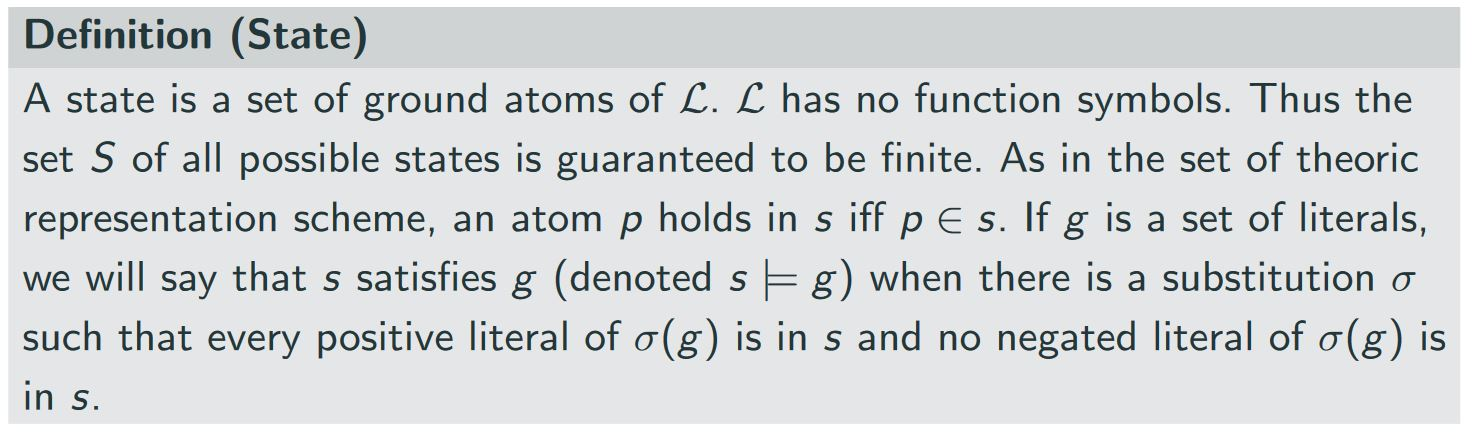
\includegraphics[keepaspectratio, width=0.90\textwidth]{images/automated_planning_state_def.jpg}
\end{center}

\end{small}
\end{frame}

\begin{frame}{States Representation Example}
\begin{small}

\begin{center}
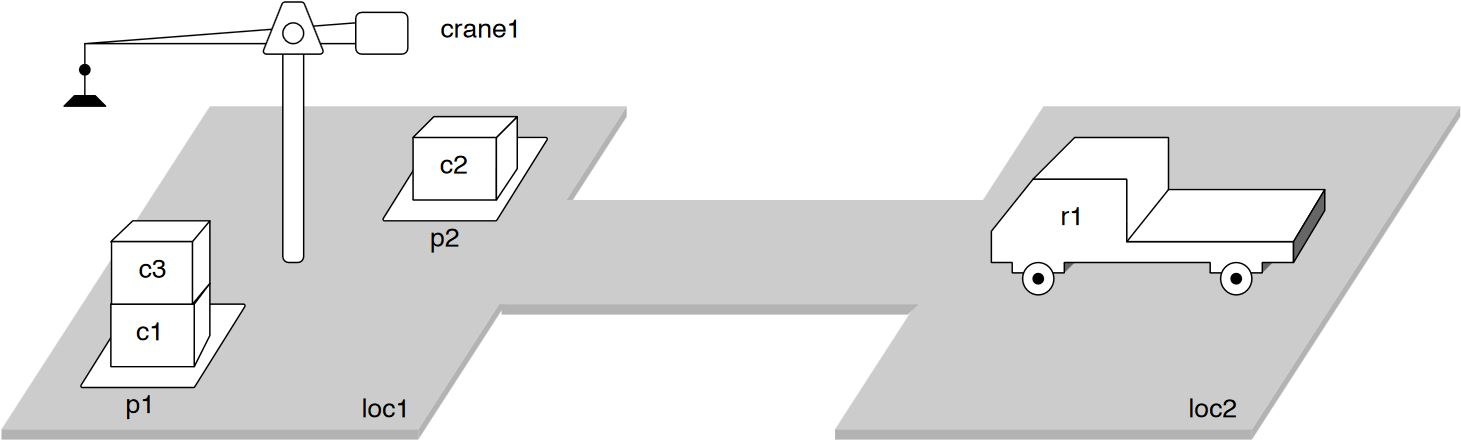
\includegraphics[keepaspectratio, width=0.90\textwidth]{images/automated_planning_example2.jpg}
\end{center}

{\footnotesize Initial state $s_0$ = {attached(p1, loc1), attached(p2, loc1) ; in(c1, p1, in(c3,p1), top(c3, p1), on(c3, c1), on(c1, pallet) in(c2, p2), top(c2, p2), on(c2,pallet),belong(crane1, loc1), empty(crane1), adjacent(loc1, loc2), adjacent(loc2, loc1), at(r1,loc2), occupied(loc2), unloaded(r1)}}
\end{small}
\end{frame}

\begin{frame}{Planning Operator Definition}
\begin{small}

The planning operators define the transition function $\gamma$ of the state transition system.

\begin{center}
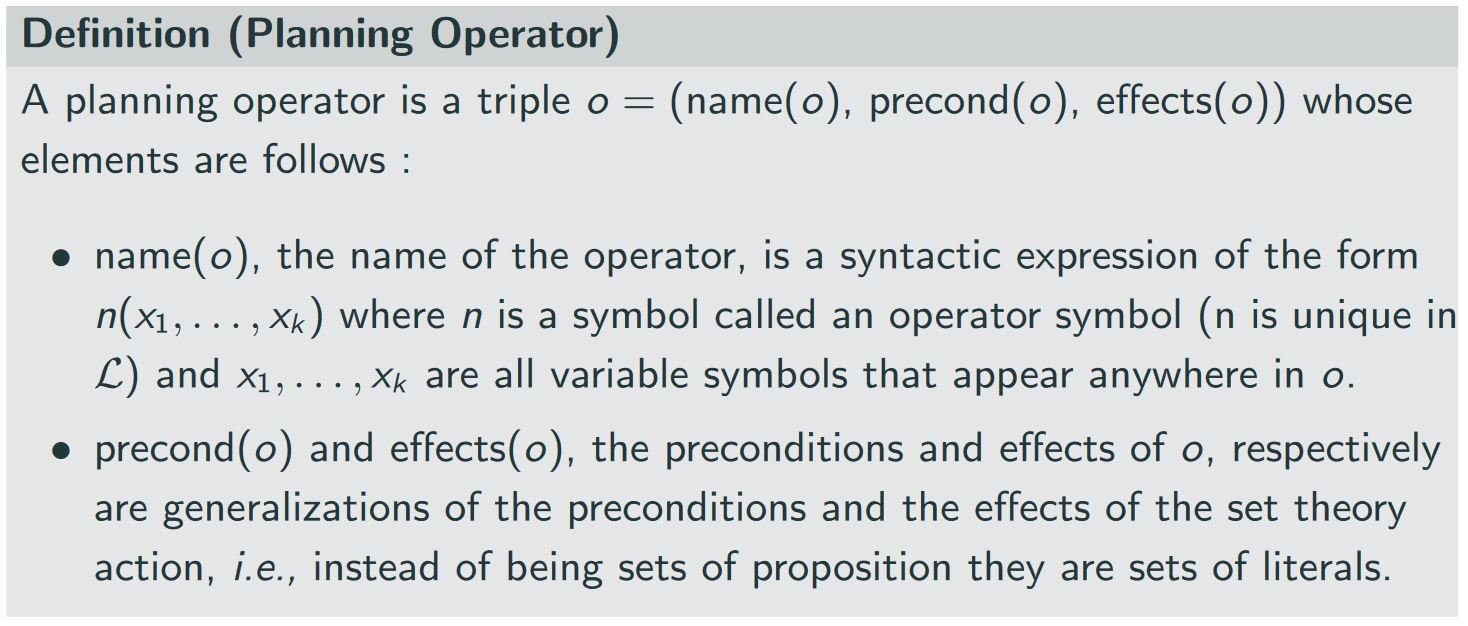
\includegraphics[keepaspectratio, width=0.90\textwidth]{images/automated_planning_operator_def.jpg}
\end{center}


\end{small}
\end{frame}

\begin{frame}{Planning Action Definition}
\begin{small}

\begin{center}
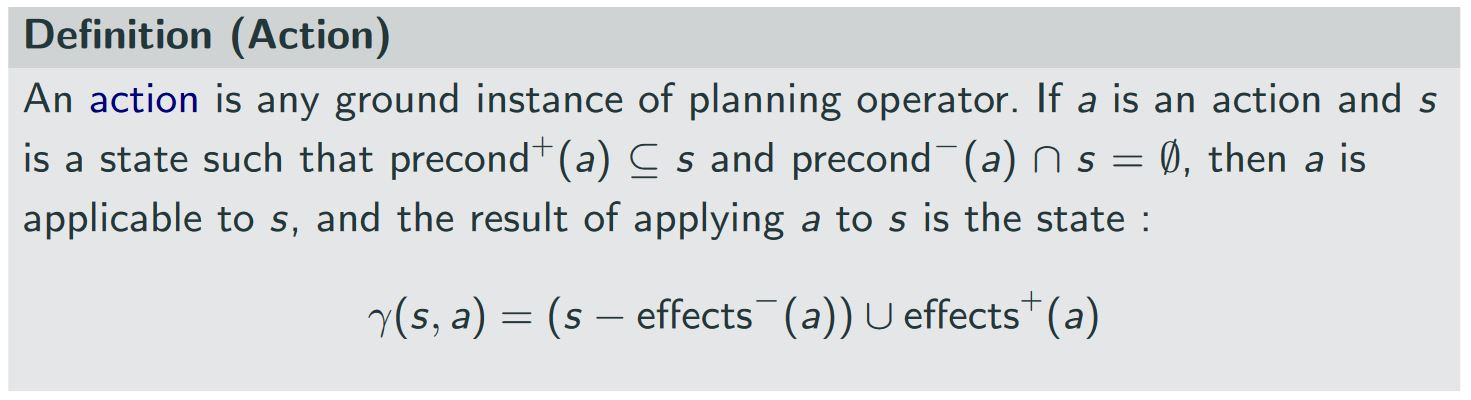
\includegraphics[keepaspectratio, width=0.90\textwidth]{images/automated_planning_action_def.jpg}
\end{center}

\end{small}
\end{frame}

\begin{frame}{Action Example}
\begin{small}

\begin{center}
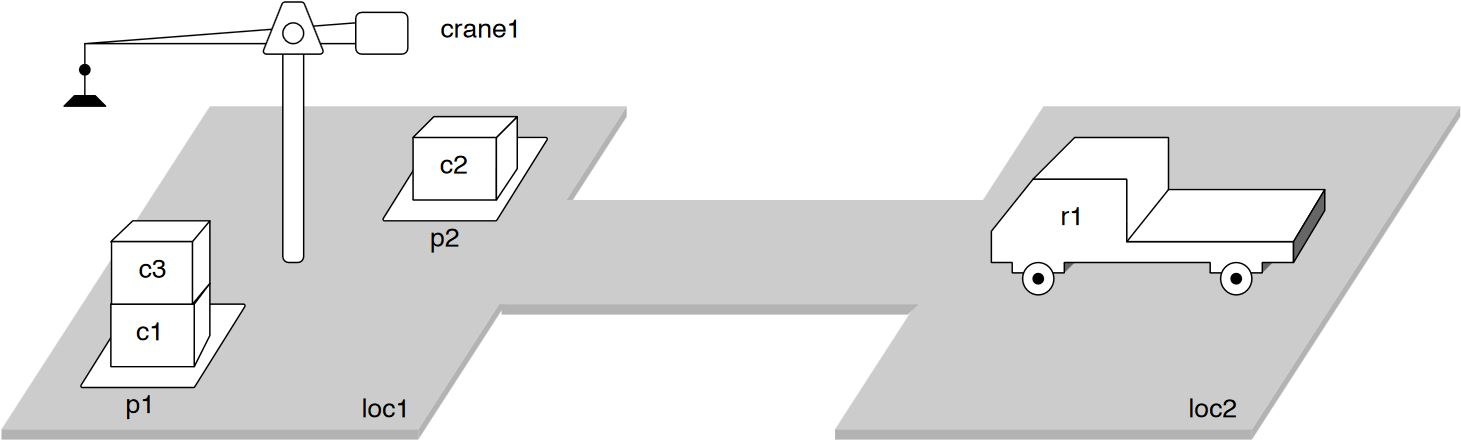
\includegraphics[keepaspectratio, width=0.75\textwidth]{images/automated_planning_example2.jpg}
\end{center}

The action $take(crane1,loc1,c3,c1,p1)$ is applicable to the state $s_0$ of the previous figure. The result is the state $s_5 = \gamma (s0,take(crane1,loc1,c3,c1,p1))$ shown by the figure below.

\begin{center}
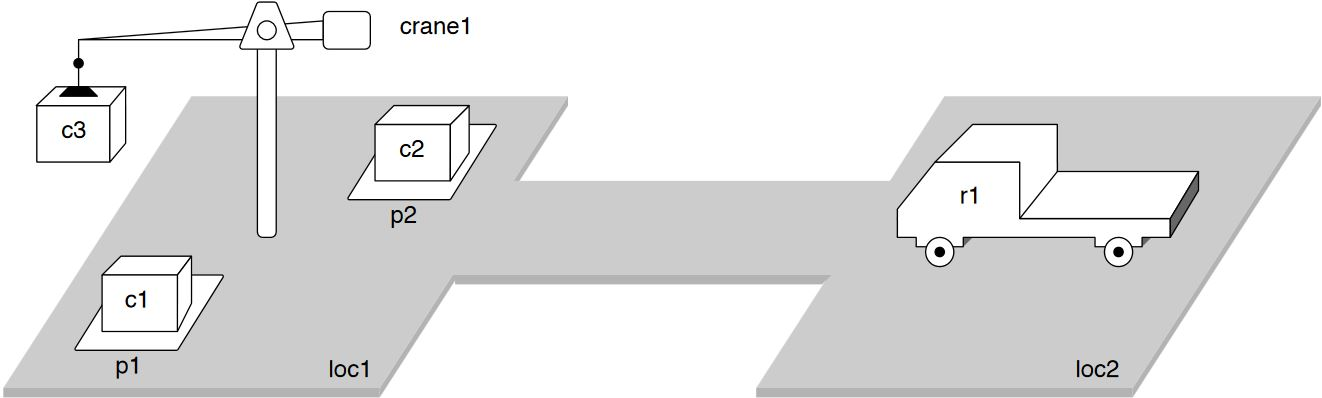
\includegraphics[keepaspectratio, width=0.75\textwidth]{images/automated_planning_example3.jpg}
\end{center}

\end{small}
\end{frame}

\begin{frame}{Classical Planning Domains Definition}
\begin{small}

\begin{center}
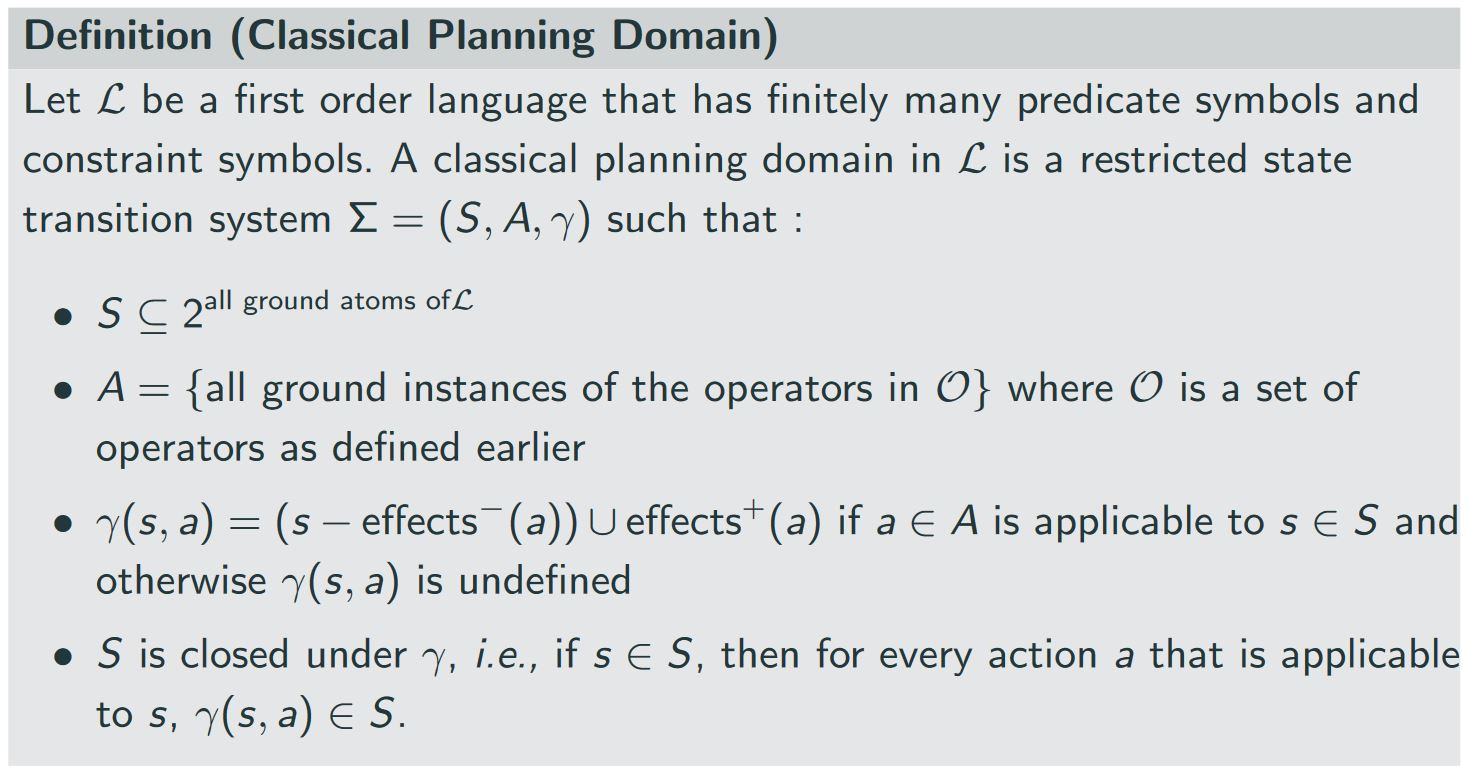
\includegraphics[keepaspectratio, width=0.90\textwidth]{images/automated_planning_classical_def.jpg}
\end{center}

\end{small}
\end{frame}

\begin{frame}{Classical Planning Problems Definition}
\begin{small}

\begin{center}
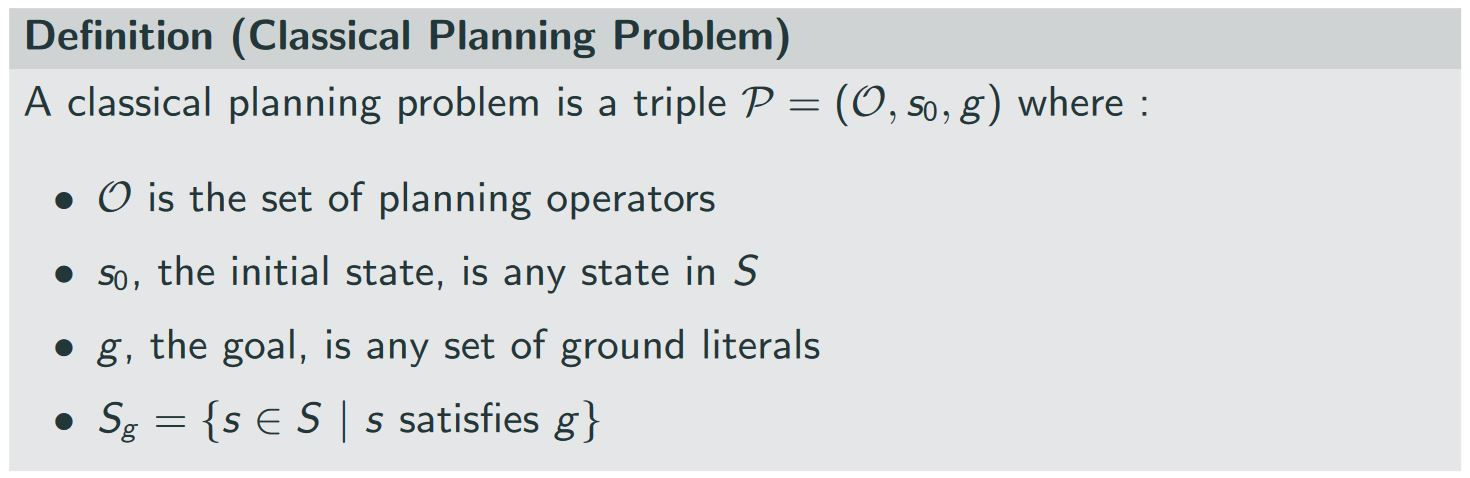
\includegraphics[keepaspectratio, width=0.90\textwidth]{images/automated_planning_classical2_def.jpg}
\end{center}

\end{small}
\end{frame}

\begin{frame}{Plan Example}
\begin{small}

\begin{center}
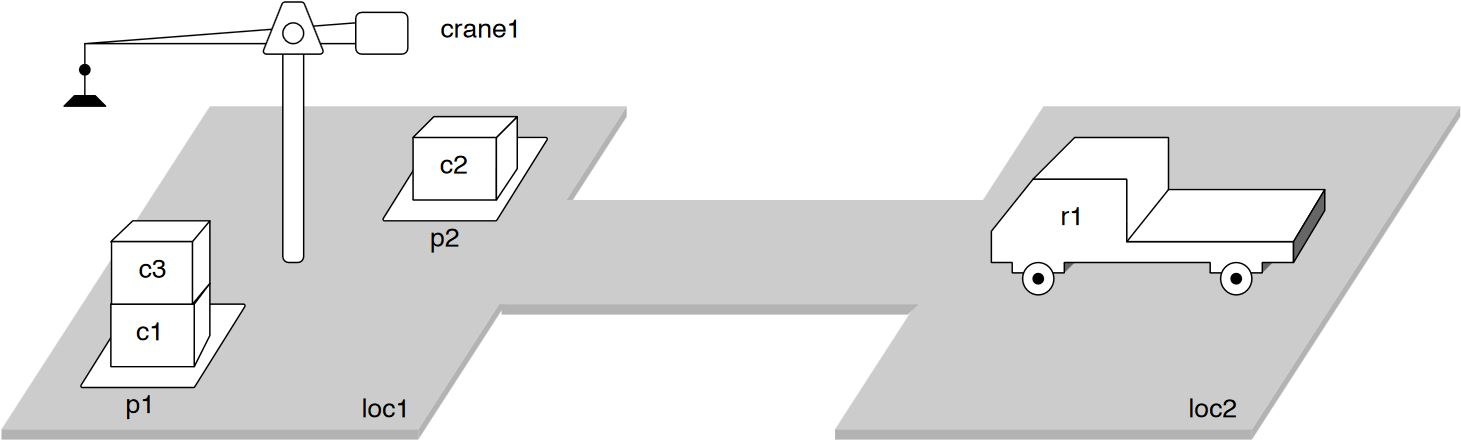
\includegraphics[keepaspectratio, width=0.75\textwidth]{images/automated_planning_example2.jpg}
\end{center}

$\pi = \{take(crane1,loc1,c3,c1,p1), move(r1,loc2,loc1), load(crane1,loc1,c3,r1)\}$

This plan is applicable to the state $s_0$ shown in previous figure producing the state $s_6$.

$g_1 = \{loaded(r1,c3), at(r1,loc1)\}$

\begin{center}
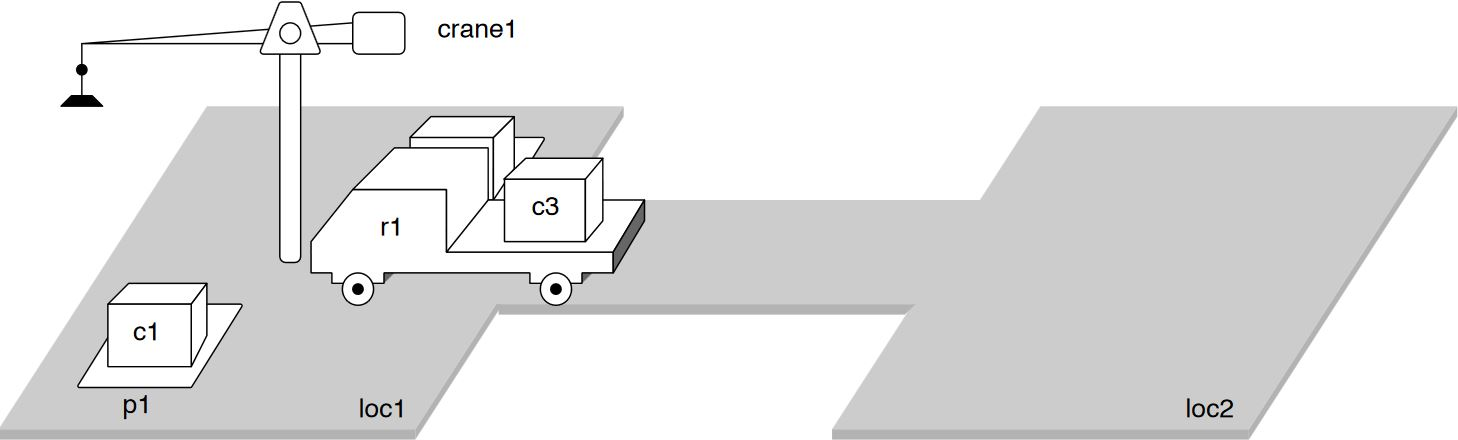
\includegraphics[keepaspectratio, width=0.75\textwidth]{images/automated_planning_example4.jpg}
\end{center}
\end{small}
\end{frame}

\begin{frame}{Extending the Classical Representation}
\begin{small}

Classical planning formalism is very restricted, extensions to it are needed in order to describe interesting domains. The most important extensions are:
\begin{itemize}
\item Typing variables;
\item Conditional Planning Operators;
\item Quantified expression;
\item Disjunctive preconditions;
\item Axiomatic Inference;
\item etc.
\end{itemize}

A planning language, called PDDL, has been developed to express all these extensions (PDDL stands for Planning Domain Description Language).
\end{small}
\end{frame}

\begin{frame}
\begin{center}
\textbf{\textcolor{CS-1light}{It's up to you !! You can do the first two practical works.}}
\end{center}
\end{frame}

\section{Solving Automated Planning Problems}

\subsection{Search problems}

\begin{frame}{Problems in AI}
\begin{small}
\begin{center}
    There are a lot of problems to solve in AI-based applications:
    
    \vspace{2mm}

    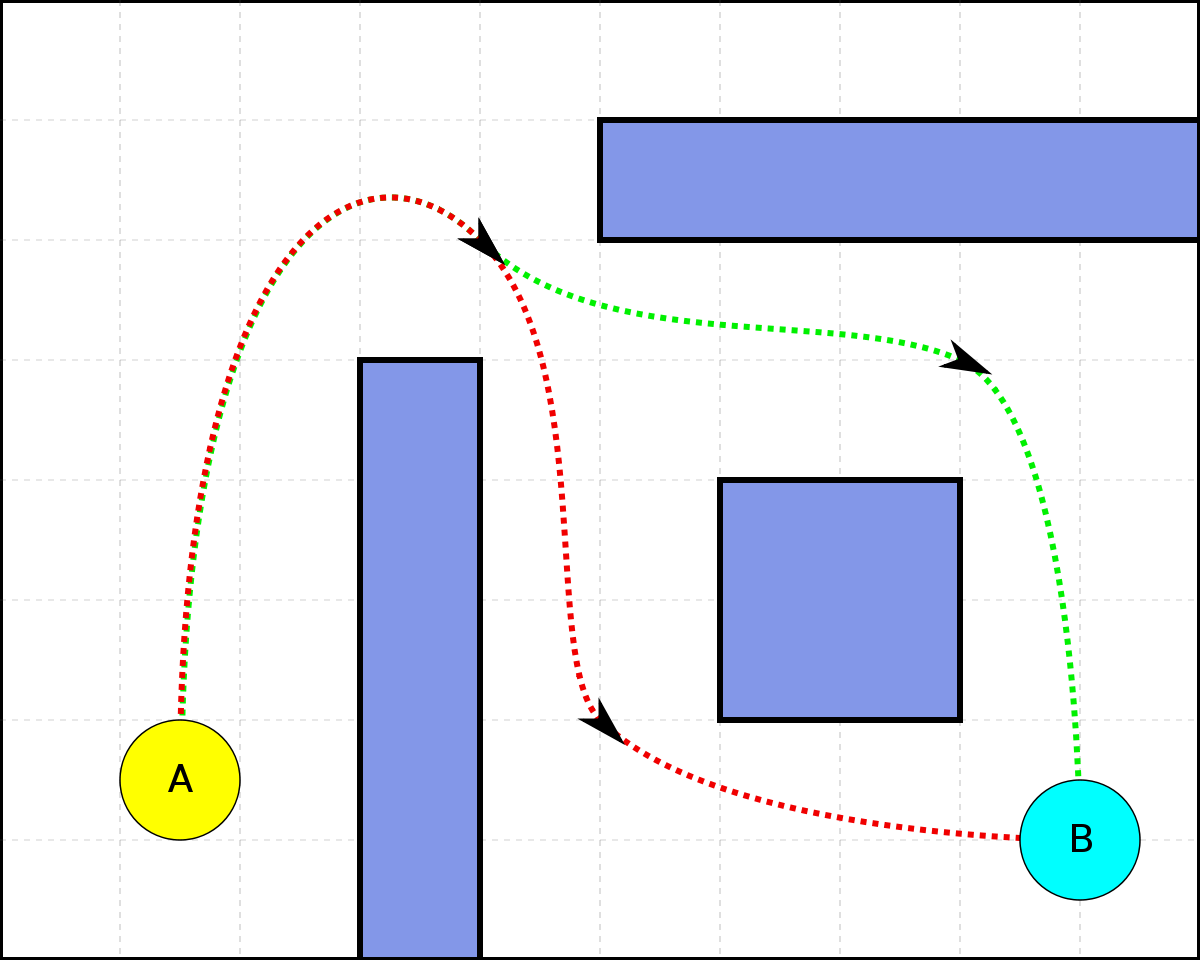
\includegraphics[keepaspectratio, height=0.15\textheight]{images/pathfinding.png}\hskip5pt
    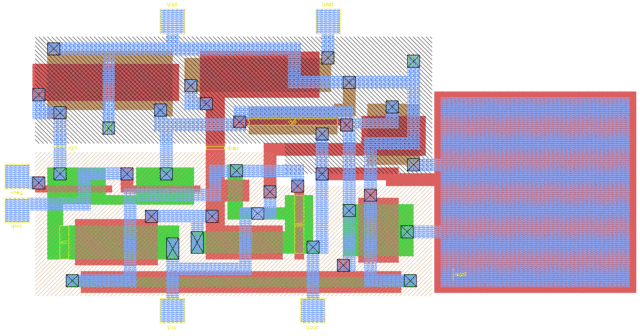
\includegraphics[keepaspectratio, height=0.15\textheight]{images/vlsi.png}\hskip5pt
    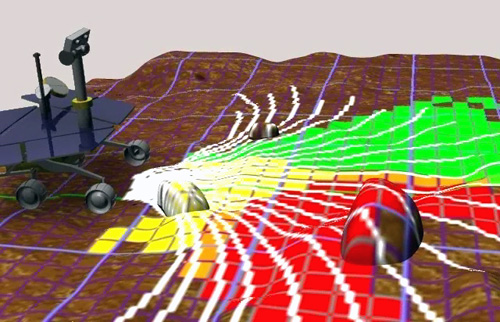
\includegraphics[keepaspectratio,height=0.15\textheight]{images/robot_nav.jpg}\hskip5pt
    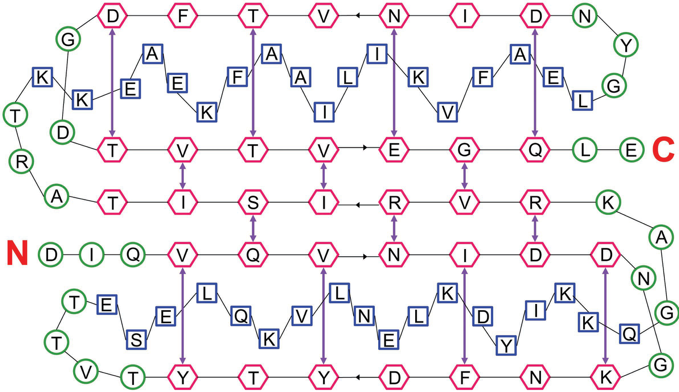
\includegraphics[keepaspectratio, height=0.15\textheight]{images/protein_design.png}
\end{center}

\textcolor{CS-2}{\textbullet} \textbf{Automatic assembly sequencing}: Find an order in which to assemble parts of an object.\\
\textcolor{CS-2}{\textbullet} \textbf{VLSI Layout problem}: Position million of components and connections on a chip to minimize area, shorten delays.\\
\textcolor{CS-2}{\textbullet} \textbf{Route finding problem}: Include tools for driving directions in websites, in-car systems, etc.\\
\textcolor{CS-2}{\textbullet} \textbf{...}
    
%\textcolor{CS-2}{\textbullet} \textbf{Travelling salesman problem}\\
%Find the shortest tour to visit each city exactly once
%\textcolor{CS-2}{\textbullet} \textbf{Robot navigation problem}\\
%\textcolor{CS-2}{\textbullet} \textbf{Protein design problem}\\
%Find a sequence of amino acids that will fold into a 3D protein with the right properties to cure some disease.

$\rightarrow$ All these kinds of problems are called \textbf{search problems}!
\end{small}
\end{frame}

\begin{frame}{Search problem}
\begin{small}

\begin{center}
    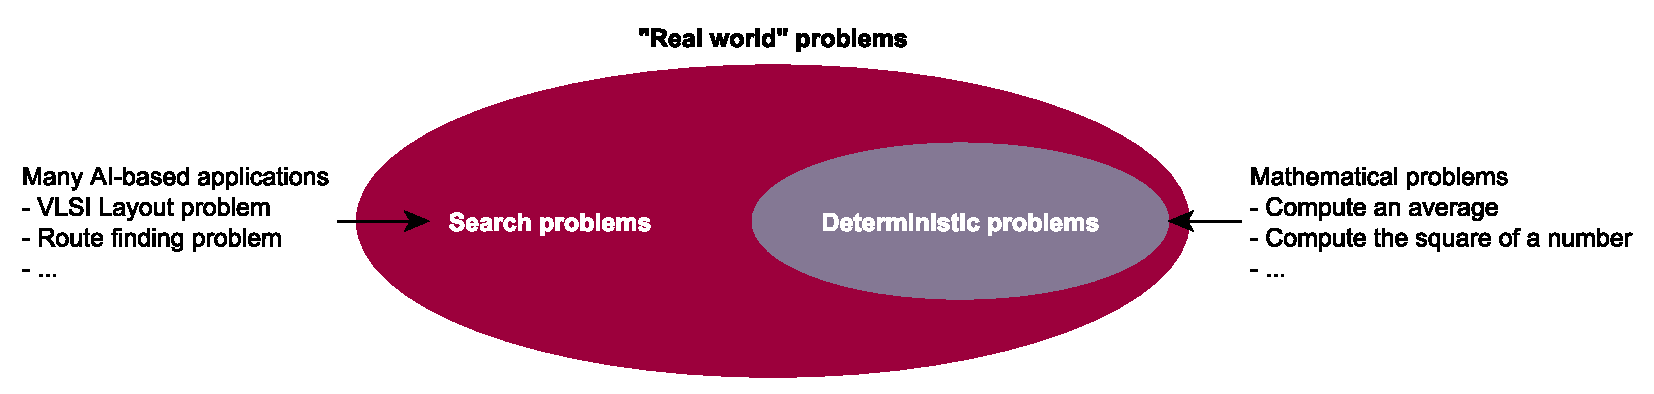
\includegraphics[keepaspectratio, width=1.0\linewidth]{images/problems.eps}
\end{center}

A problem is a \textbf{search problem} if there's an \textbf{algorithmic way} to find the solution.
\vspace{-3mm}
\begin{itemize}
    \item It cannot be solve by deterministic procedure.
    \item It can only be solved by searching for a solution and the success is not guarenteed.
\end{itemize}
\end{small}
\end{frame}


\begin{frame}{Search problem}
\begin{small}

A \textbf{search problem} is defined by:
\vspace{-3mm}
\begin{itemize}
    \item A \textbf{state space}: Set of all possible states of the problem.
    \item A \textbf{start state}: The initial state of the problem.
    \item A \textbf{goal state}: The goal state to reach to solve the problem.
    \item A \textbf{solution plan}: The sequence of actions to reach the goal state.
\end{itemize}

\vspace{-2mm}

\emph{Note:} Search problems can be often represented using graphs.

\begin{center}
    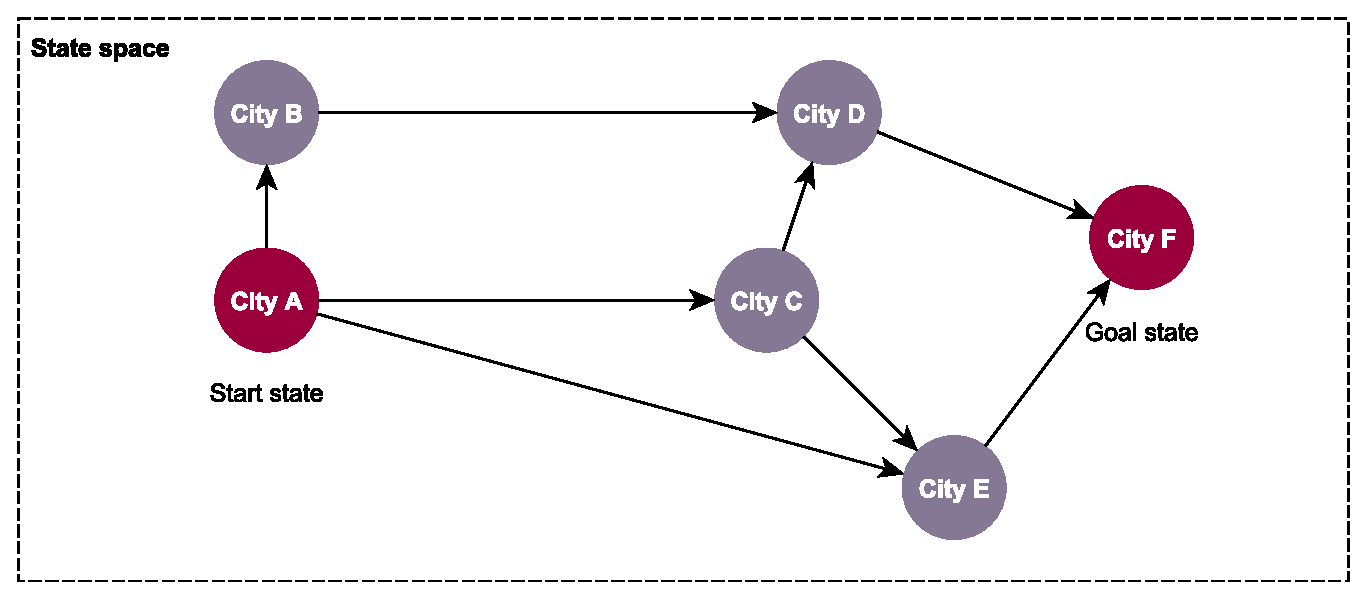
\includegraphics[keepaspectratio, width=0.75\textwidth]{images/h_example_0.eps}
\end{center}

\end{small}
\end{frame}

\begin{frame}{Informed Search Algorithms}
\begin{small}
\begin{center}
    To solve search problems, one must use \textbf{search algorithms}!
    
    \vspace{2mm}

    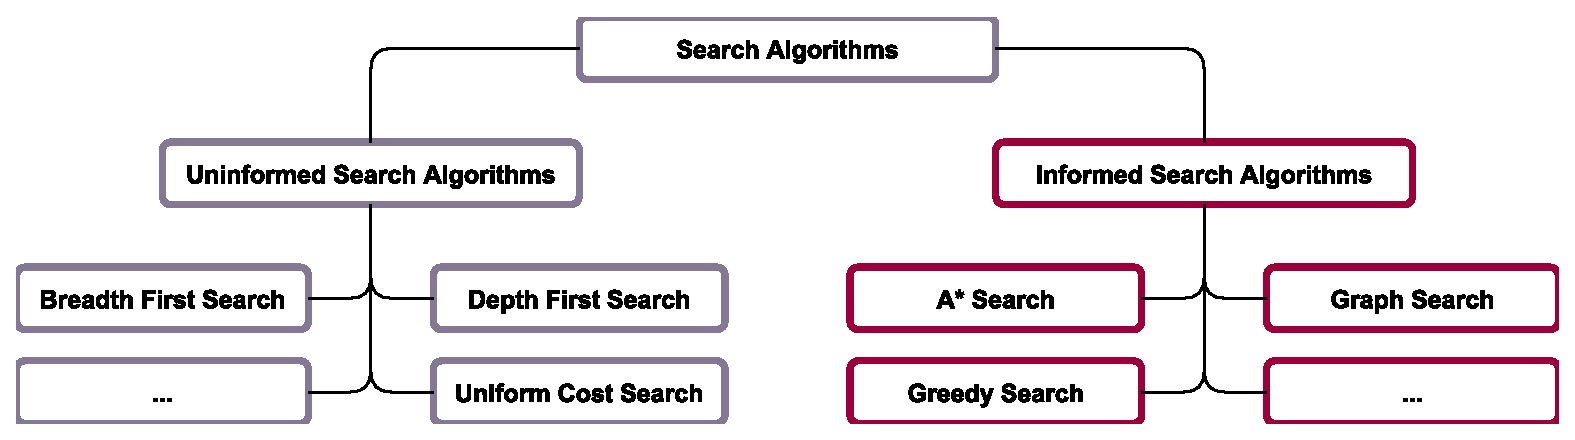
\includegraphics[keepaspectratio, width=1.00\textwidth]{images/search_algorithms.eps}\\
    \textcolor{CS-2}{No additional information} \hfill \textcolor{CS-1}{Receive additional information}
\end{center}

$\rightarrow$ To \textbf{solve large problems} with large number of possible states, \textbf{problem-specific knowledge} needs to be added to increase the efficiency of search algorithms. This knowledge is obtained by a \textbf{heuristic} function.
\end{small}
\end{frame}

\subsection{Heuristics}
% Vocabulary, What is a heuristic, How can they help algorithms, popular heursitics

\begin{frame}{What is a heuristic ?}
\begin{small}
\only<1>{
\textbf{Definition}\\
A \textbf{heuristic function}, also called simply a heuristic, is a function that ranks alternatives in search algorithms: It estimates how close a state is to the goal state \cite{Osti1984}.

\textbf{Example:} \texttt{SUM} heuristic (\emph{sum the cost of all distance to the goal})\\
\begin{center}
    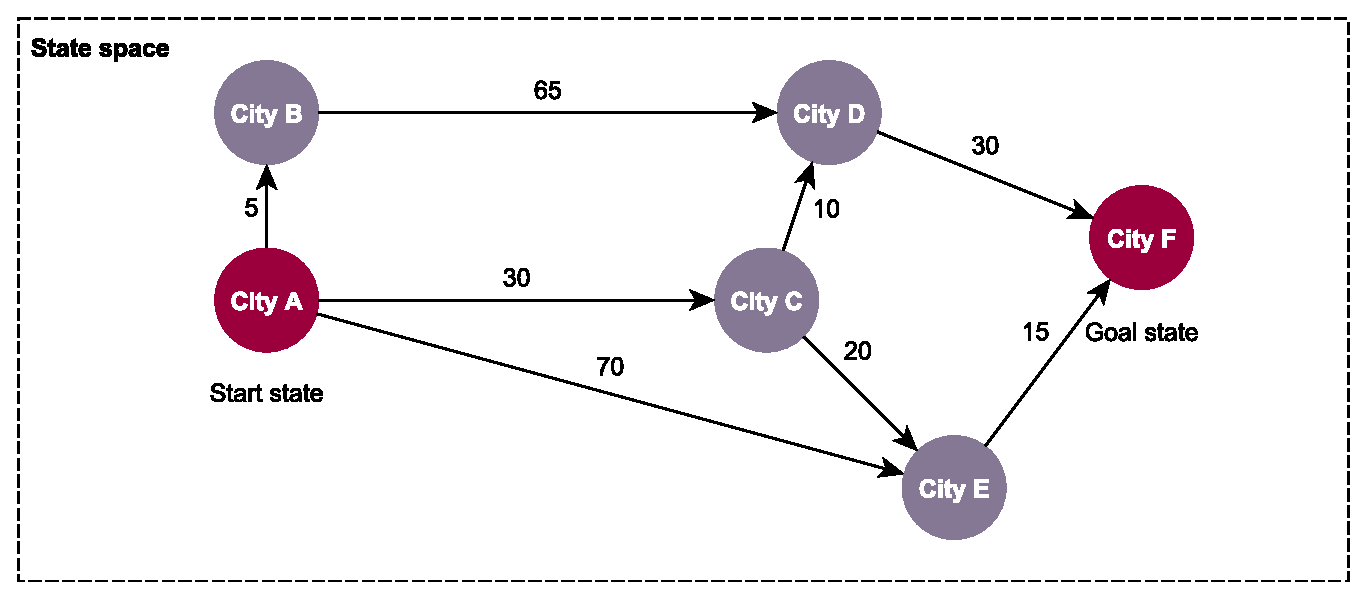
\includegraphics[keepaspectratio, width=0.9\textwidth]{images/h_example_1.eps}
\end{center}
}
\only<2>{
\textbf{Definition}\\
A \textbf{heuristic function}, also called simply a heuristic, is a function that ranks alternatives in search algorithms: It estimates how close a state is to the goal state \cite{Osti1984}.

\textbf{Example:} \texttt{SUM} heuristic (\emph{sum the cost of all distance to the goal})\\
\begin{center}
    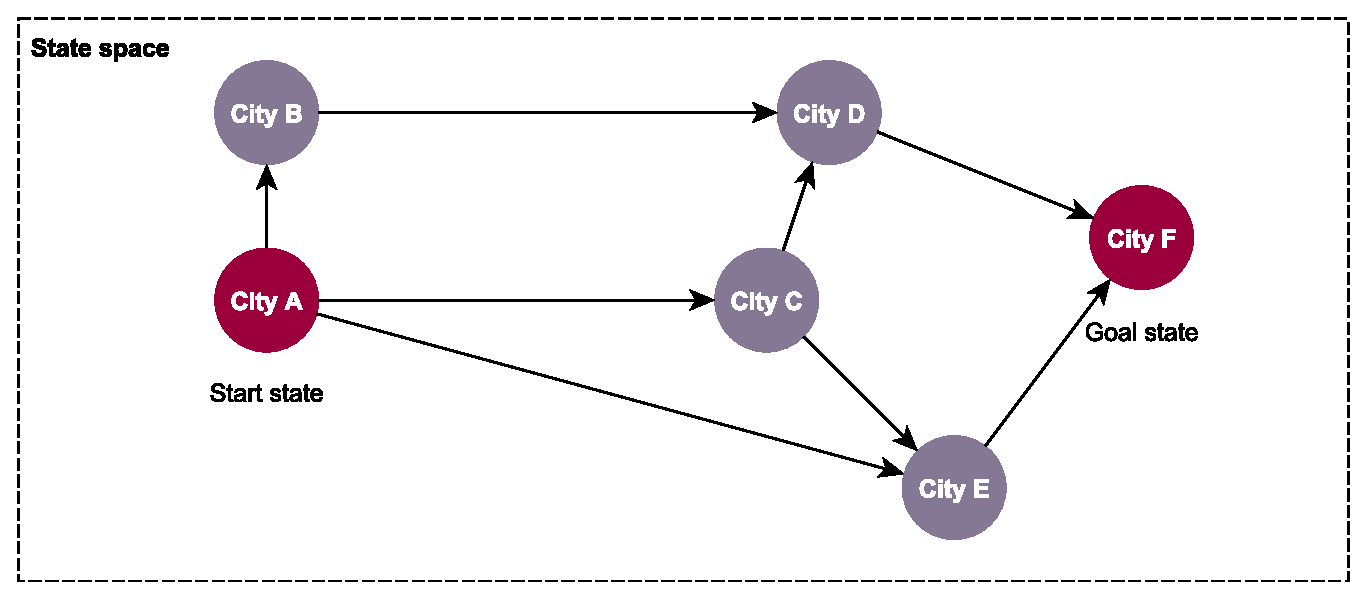
\includegraphics[keepaspectratio, width=0.9\textwidth]{images/h_example_0.eps}
\end{center}
}
\only<3>{
\textbf{Definition}\\
A \textbf{heuristic function}, also called simply a heuristic, is a function that ranks alternatives in search algorithms: It estimates how close a state is to the goal state \cite{Osti1984}.

\textbf{Example:} \texttt{SUM} heuristic (\emph{sum the cost of all distance to the goal})\\
\begin{center}
    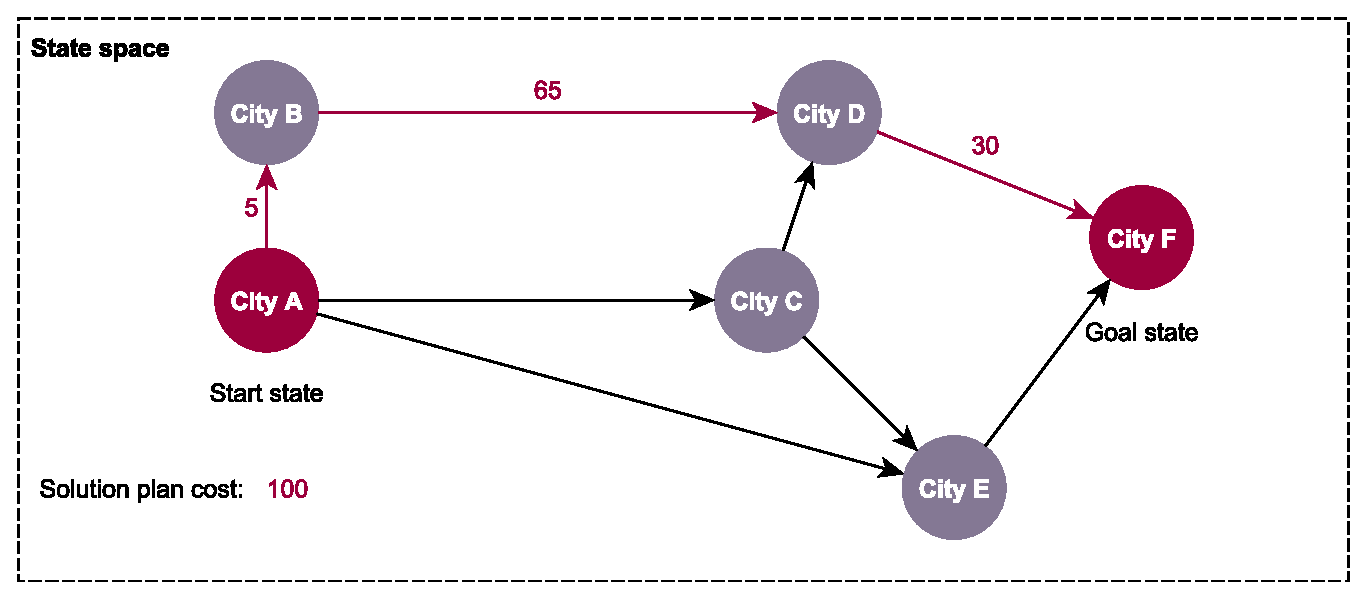
\includegraphics[keepaspectratio, width=0.9\textwidth]{images/h_example_2.eps}
\end{center}
}
\only<4>{
\textbf{Definition}\\
A \textbf{heuristic function}, also called simply a heuristic, is a function that ranks alternatives in search algorithms: It estimates how close a state is to the goal state \cite{Osti1984}.

\textbf{Example:} \texttt{SUM} heuristic (\emph{sum the cost of all distance to the goal})\\
\begin{center}
    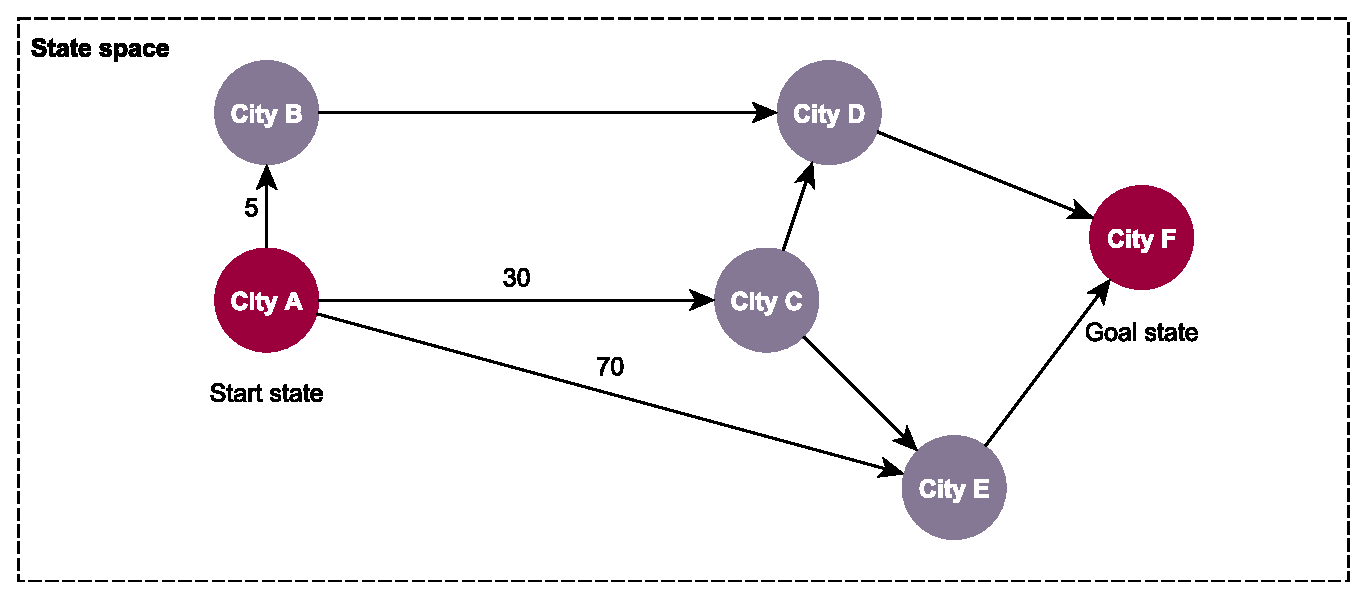
\includegraphics[keepaspectratio, width=0.9\textwidth]{images/h_example_1bis.eps}
\end{center}
}
\only<5>{
\textbf{Definition}\\
A \textbf{heuristic function}, also called simply a heuristic, is a function that ranks alternatives in search algorithms: It estimates how close a state is to the goal state \cite{Osti1984}.

\textbf{Example:} \texttt{SUM} heuristic (\emph{sum the cost of all distance to the goal})\\
\begin{center}
    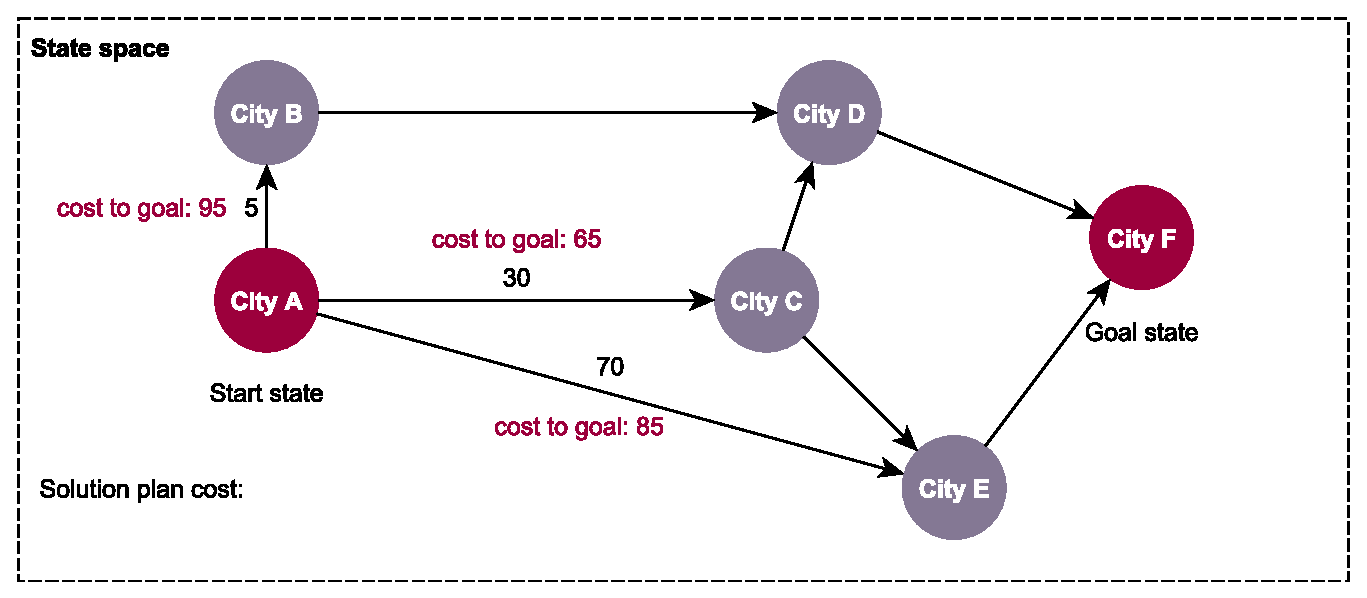
\includegraphics[keepaspectratio, width=0.9\textwidth]{images/h_example_3.eps}
\end{center}
}
\only<6>{
\textbf{Definition}\\
A \textbf{heuristic function}, also called simply a heuristic, is a function that ranks alternatives in search algorithms: It estimates how close a state is to the goal state \cite{Osti1984}.

\textbf{Example:} \texttt{SUM} heuristic (\emph{sum the cost of all distance to the goal})\\
\begin{center}
    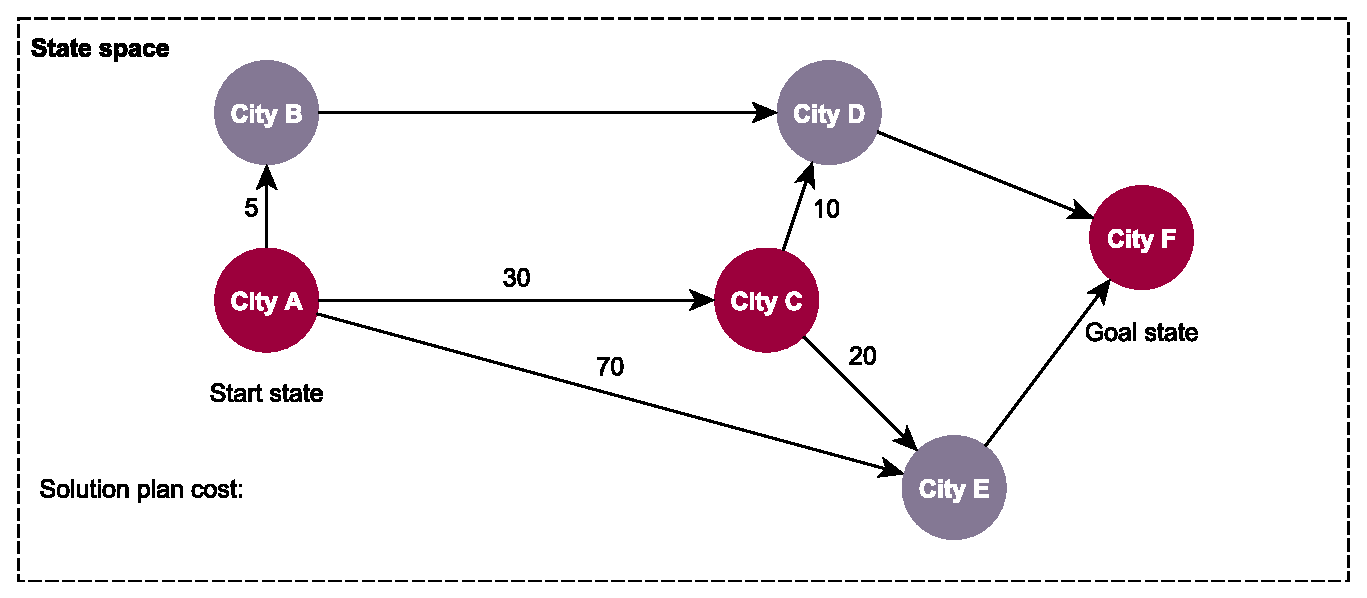
\includegraphics[keepaspectratio, width=0.9\textwidth]{images/h_example_4.eps}
\end{center}
}
\only<7>{
\textbf{Definition}\\
A \textbf{heuristic function}, also called simply a heuristic, is a function that ranks alternatives in search algorithms: It estimates how close a state is to the goal state \cite{Osti1984}.

\textbf{Example:} \texttt{SUM} heuristic (\emph{sum the cost of all distance to the goal})\\
\begin{center}
    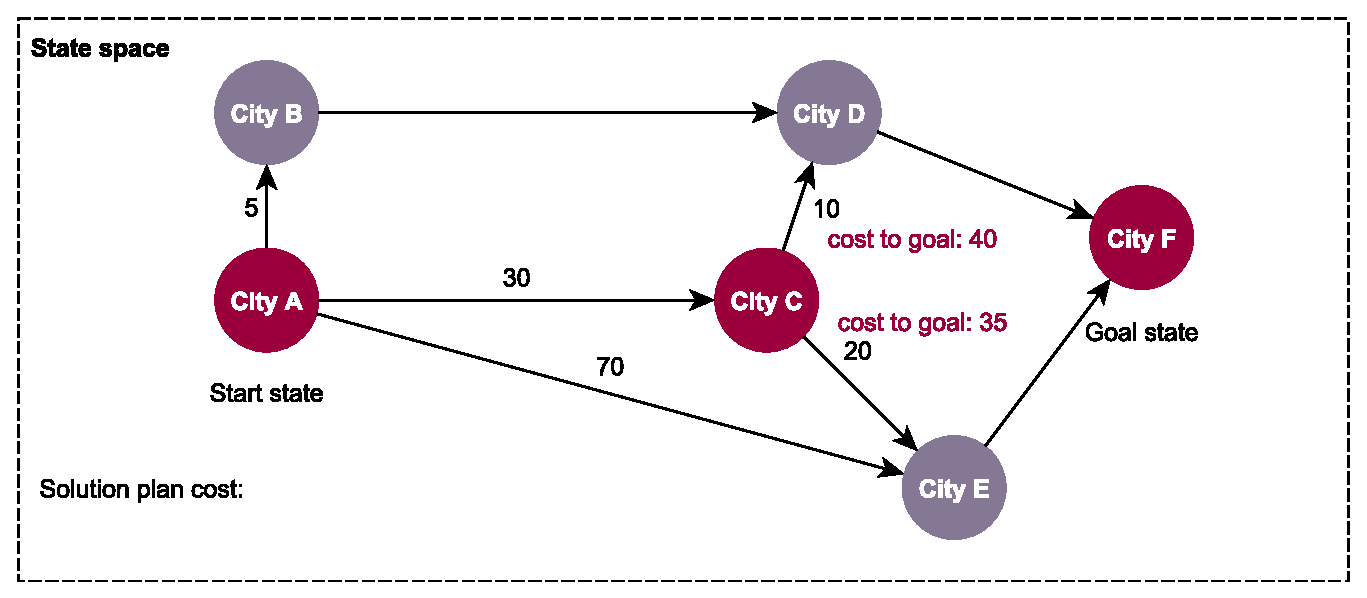
\includegraphics[keepaspectratio, width=0.9\textwidth]{images/h_example_5.eps}
\end{center}
}
\only<8>{
\textbf{Definition}\\
A \textbf{heuristic function}, also called simply a heuristic, is a function that ranks alternatives in search algorithms: It estimates how close a state is to the goal state \cite{Osti1984}.

\textbf{Example:} \texttt{SUM} heuristic (\emph{sum the cost of all distance to the goal})\\
\begin{center}
    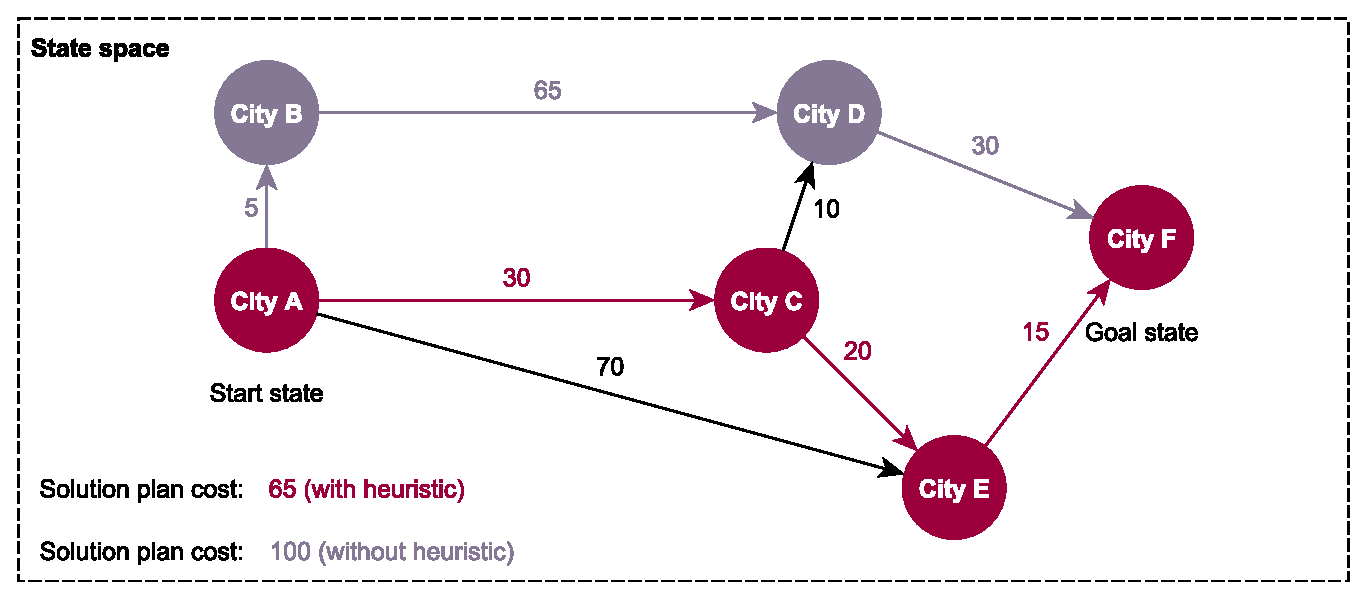
\includegraphics[keepaspectratio, width=0.9\textwidth]{images/h_example_6.eps}
\end{center}
}

\end{small}
\end{frame}

\begin{frame}{Admissible heuristic}
\begin{small}
\textbf{Admissible heuristic definition} \cite{Russell2002}\\
A heuristic function is said to be \textbf{admissible} if it never overestimates the cost of reaching the goal. The cost it estimates to reach the goal is not higher than the lowest possible cost from the current state: It is \textbf{optimistic}.

\textbf{Formulation}\\
$n$ is a node wich represents a state\\
$h$ is a heuristic function\\
$h(n)$ is cost indicated by $h$ to reach a goal from $n$\\
$h'(n)$ is the optimal cost to reach a goal from $n$\\

\begin{center}
   \textcolor{CS-1}{$h(n)$ is admissible if, $\forall n$
   $h(n) \leq h'(n)$}
\end{center}
\end{small}
\end{frame}

\begin{frame}{Consistent heuristic}
\begin{small}
\textbf{Consistent heuristic definition} \cite{Russell2002}\\
A heuristic function is said to be \textbf{consistent}, if its estimate is always less than or equal to the estimated distance from any neighbouring state to the goal, plus the cost of reaching that neighbour state.

\begin{minipage}[t]{0.65\linewidth}\vspace{0pt}%	
\textbf{Formulation}\\
$n$ is a node wich represents a state\\
$h$ is a heuristic function\\
$p$ is any descendant of $n$\\
$g$ is any goal node\\
$c(n,p)$ is the cost of reaching node $p$ from $n$\\
\end{minipage}
\hskip5pt
\begin{minipage}[t]{0.30\linewidth}\vspace{0pt}%	
    \begin{center}
    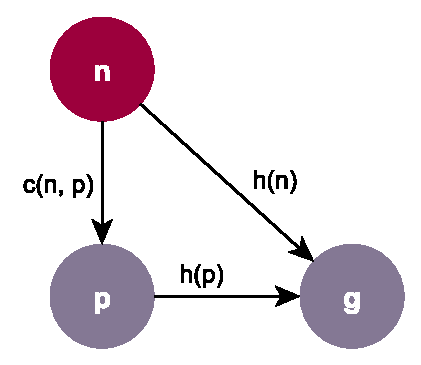
\includegraphics[keepaspectratio, width=0.8\textwidth]{images/consistent_h.eps}
    \end{center}
\end{minipage}

\begin{center}
    \textcolor{CS-1}{$h(n) \leq c(n,p) + h(p)$ and 
    $h(g) = 0$}
\end{center}

%For every node $n$ and each successor $p$ of $n$, the estimated cost of reaching the goal from $n$ is no greater than the step cost of getting to $p$ plus the estimated cost of reaching the goal from $p$.

\emph{Note:} A consistent heuristic is also admissible (the reverse is not always true) \cite{Edelkamp2011}.
\end{small}
\end{frame}

\subsection{Informed Search Algorithms}

\begin{frame}{Search process in search algorithms}
\begin{small}

The \textbf{search process} in a search algorithms consists in \textbf{exploring the state space} from the initial state to the goal state.

\textbf{Search algorithms} uses a \textbf{search tree} which represents the exploration trace:
\vspace{-3mm}
\begin{itemize}
    \item \textbf{Search tree} is built during the search process.
    \item \textbf{Branches} correspond to explored paths and \textbf{nodes} to the exploration fringe.
\end{itemize}

\begin{center}
    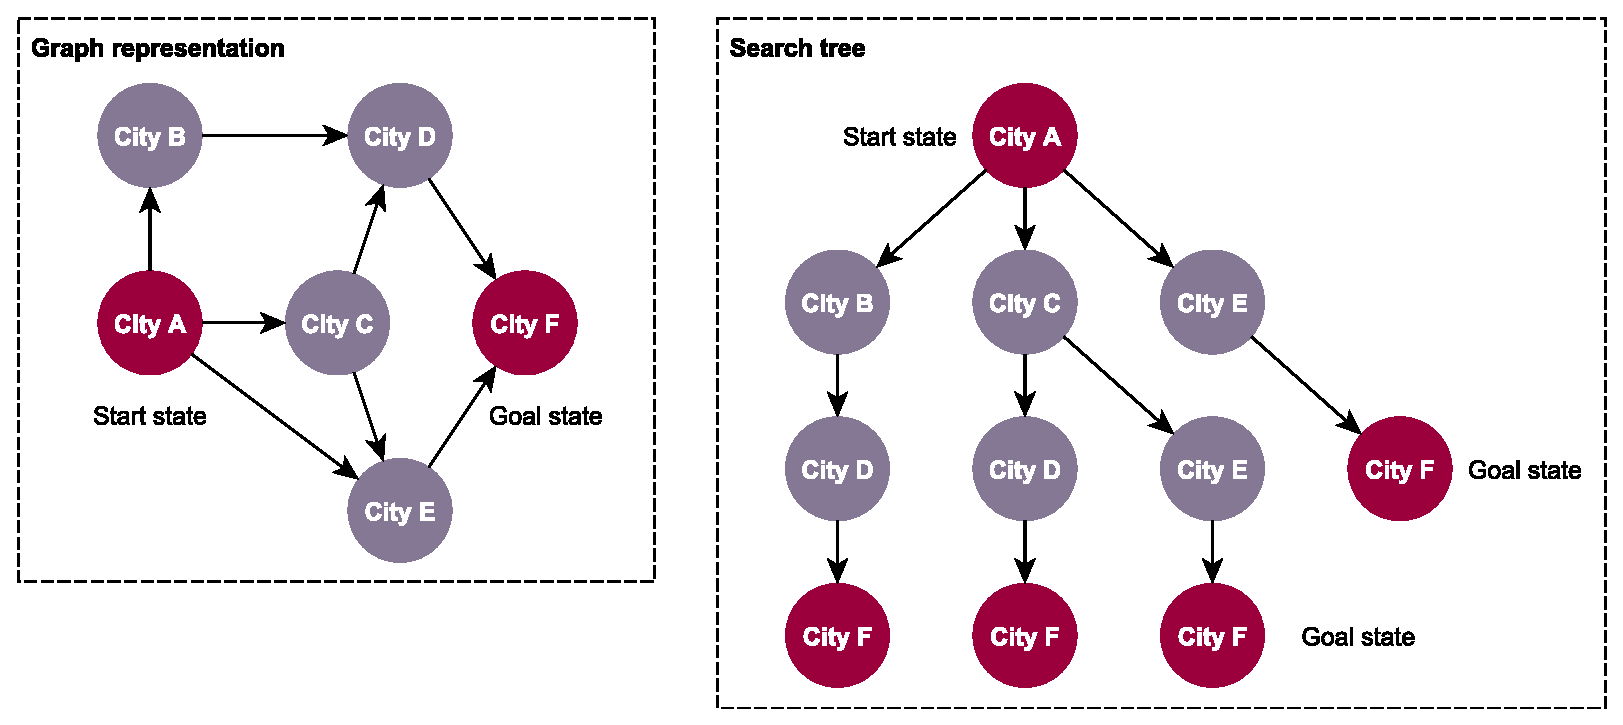
\includegraphics[keepaspectratio, width=0.9\linewidth]{images/tree.eps}
\end{center}
\end{small}
\end{frame}

\begin{frame}{Search tree expanding rules}
\begin{small}
Search algorithms differ in the way they determine the next node to expand in the search tree:

\begin{itemize}
    \item \textbf{Uninformed Search}: Rigid procedure with no knowledge of the cost of a given node to the goal.
    \item \textbf{Informed Search}: Knowledge of the worth of expanding a node $n$ is given in the form of an evaluation function $f(n)$, which assigns a real number to each node. Mostly, $f(n)$ includes as a component a heuristic function $h(n)$, which estimates the costs of the cheapest path from $n$ to the goal.\\
\end{itemize}

\end{small}
\end{frame}

\begin{frame}{Best-First Search}
\begin{small}

\textbf{Best-first search} is an instance of the general \texttt{Tree-Search} algorithm in which \emph{frontier} is a priority queue ordered by an evaluation function $f$.

$\rightarrow$ Best-first search expands the node with the \textbf{“best”} $f$-value first. It could allow revising previous nodes.

\textbf{function} \texttt{TREE-SEARCH}(\emph{problem}):\\

\begin{minipage}{0.20\linewidth}\vspace{0pt}%
\end{minipage}
\hskip10pt
\begin{minipage}{0.80\linewidth}\vspace{0pt}%	
\begin{algorithm}[H]
    \KwData{\emph{frontier}, an ordered priority queue}
	initialize the \emph{frontier} using the initial state of \emph{problem}\;
	\While{\emph{frontier} \textbf{is not} empty}
 	{
  		choose a leaf node with the best \emph{f}-value and remove it from the \emph{frontier}\;
  		\If{the node contains a goal state}
  		{
  		    \textbf{return} the corresponding solution\;
  		}
  		expand the chosen node, adding the resulting nodes to the \emph{frontier}\;
  	}
  	\textbf{return} failure\;
\end{algorithm}
\end{minipage}

\end{small}
\end{frame}

\begin{frame}{Greedy Best First Search}
\begin{small}

A \textbf{best-first search} using $f(n) = h(n)$ as the evaluation function is called a \textbf{greedy search}.

$\rightarrow$ Greedy best-first search expands the nodes estimated to be closest to goal.

\end{small}
\end{frame}

\begin{frame}{Greedy Best First Search properties}
\begin{small}
\begin{itemize}
    \item A good heuristic might reduce search time drastically.
    \item Non-optimal (\emph{it not guarantees to return the best solution}).
    \item Incomplete (\emph{it not guarantees to return a correct answer for any arbitrary input}); Can be stuck in a loop.
    \item Keep all nodes in memory.
\end{itemize}

\begin{center}
    \textbf{Can we do better?}
\end{center}

\end{small}
\end{frame}

\begin{frame}{A*: Minimization of the estimated path costs}
\begin{small}
\textbf{A*} combines the \textbf{greedy search} with the \textbf{uniform-search strategy}: Always expand node with lowest $f(n)$ first. \\

\vspace{2mm}

\hskip20pt $g(n) = $ actual cost from the initial state to n\\
\hskip20pt $h(n) = $ estimated cost from n to the next goal\\
\hskip20pt $f(n) = g(n) + h(n)$ the estimated cost of the cheapest solution through $n$\\

\vspace{2mm}

A* requires that $h$ is admissible to be \textbf{complete} and \textbf{optimal}.
\end{small}
\end{frame}

\begin{frame}{A* Search}
\begin{small}

\textbf{function} \texttt{AStar}(\emph{problem}):\\

\begin{minipage}{0.10\linewidth}\vspace{0pt}%
\end{minipage}
\hskip10pt
\begin{minipage}{0.90\linewidth}\vspace{0pt}%	
\begin{algorithm}[H]
    \KwData{\emph{OPEN} and \emph{CLOSED}, two lists}
	Place the starting node into \emph{OPEN} using the initial state of \emph{problem}\;
	\While{\emph{OPEN} \textbf{is not} empty}
 	{
  		Select the node $p$ from \emph{OPEN} which has the smallest value of evaluation function $f(n) = g(n) + h(n)$\;
  		\If{$p$ \textbf{is} a goal state}
  		{
  		    \textbf{return} the corresponding solution\;
  		}
  		Expand node $n$ and generate all of its $p$ successors, and put $n$ into \emph{CLOSED}\;
  		\ForEach{$p$ successors}
  		{
  		    Check whether $p$ is already in the \emph{OPEN} or \emph{CLOSED}, if not then compute evaluation function for $p$ and place into \emph{OPEN}\;
  		}
  	}
  	\textbf{return} failure\;
\end{algorithm}
\end{minipage}

\end{small}
\end{frame}

\begin{frame}{A* Search example (8-puzzle problem)}
\begin{small}

\only<1> {
\begin{center}
    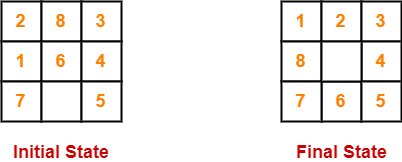
\includegraphics[keepaspectratio, width=0.60\linewidth]{images/A-Algorithm-Problem-01.png}
\end{center}

Find the most cost-effective path to reach the final state from initial state using A* Algorithm.

Consider:
\begin{itemize}
    \item $g(n) =$ Depth of node
    \item $h(n) =$ Number of misplaced tiles.
\end{itemize}
}

\only<2> {
\begin{center}
    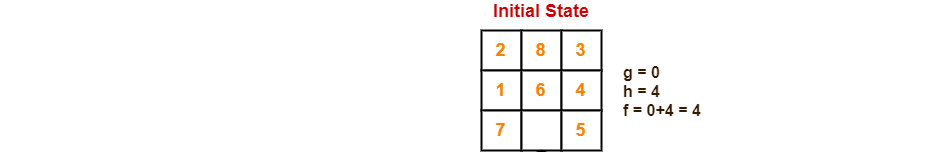
\includegraphics[keepaspectratio, width=0.75\linewidth]{images/Solve-Problem-01-01.png}
\end{center}
}

\only<3> {
\begin{center}
    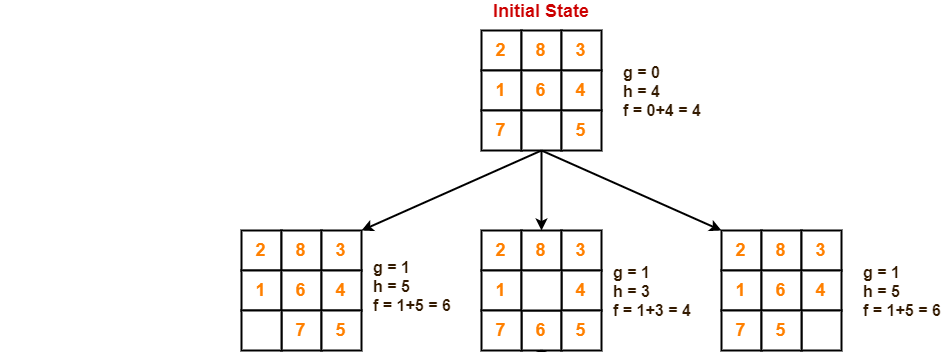
\includegraphics[keepaspectratio, width=0.75\linewidth]{images/Solve-Problem-01-02.png}
\end{center}
}

\only<4> {
\begin{center}
    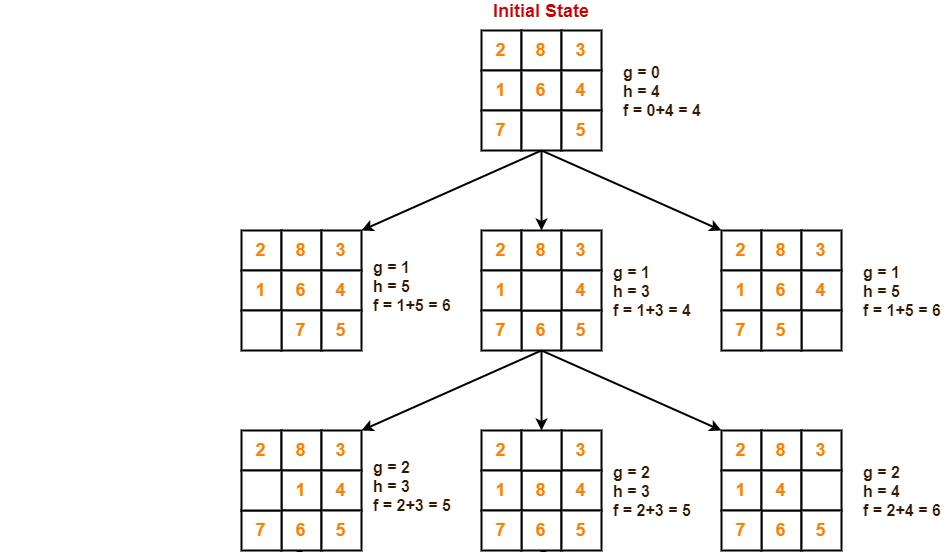
\includegraphics[keepaspectratio, width=0.75\linewidth]{images/Solve-Problem-01-03.png}
\end{center}
}

\only<5> {
\begin{center}
    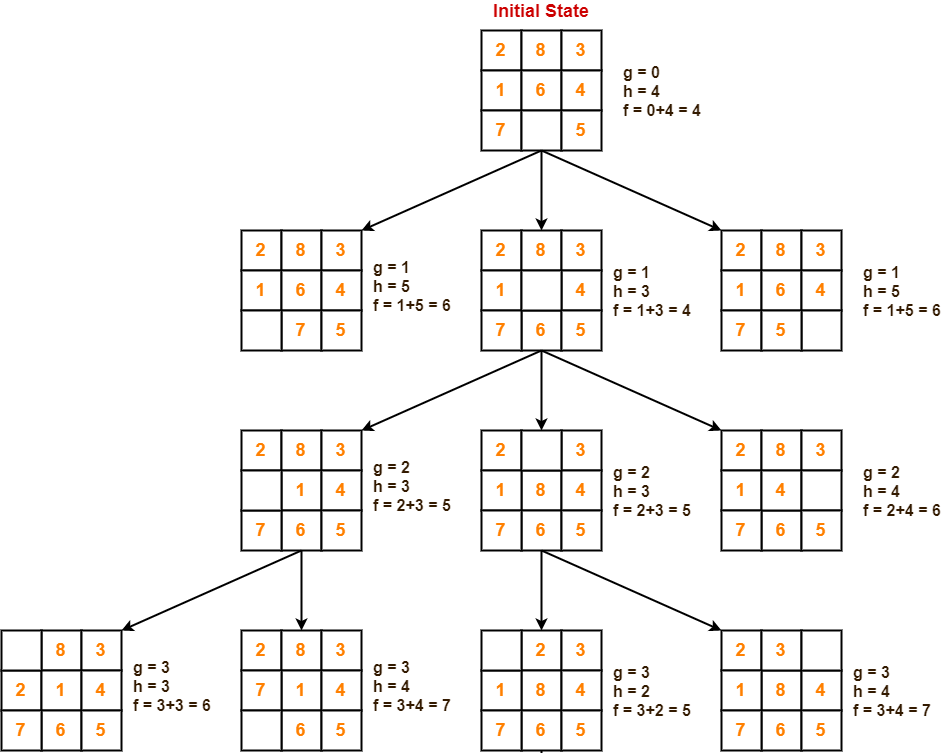
\includegraphics[keepaspectratio, width=0.75\linewidth]{images/Solve-Problem-01-04.png}
\end{center}
}

\only<6> {
\begin{center}
    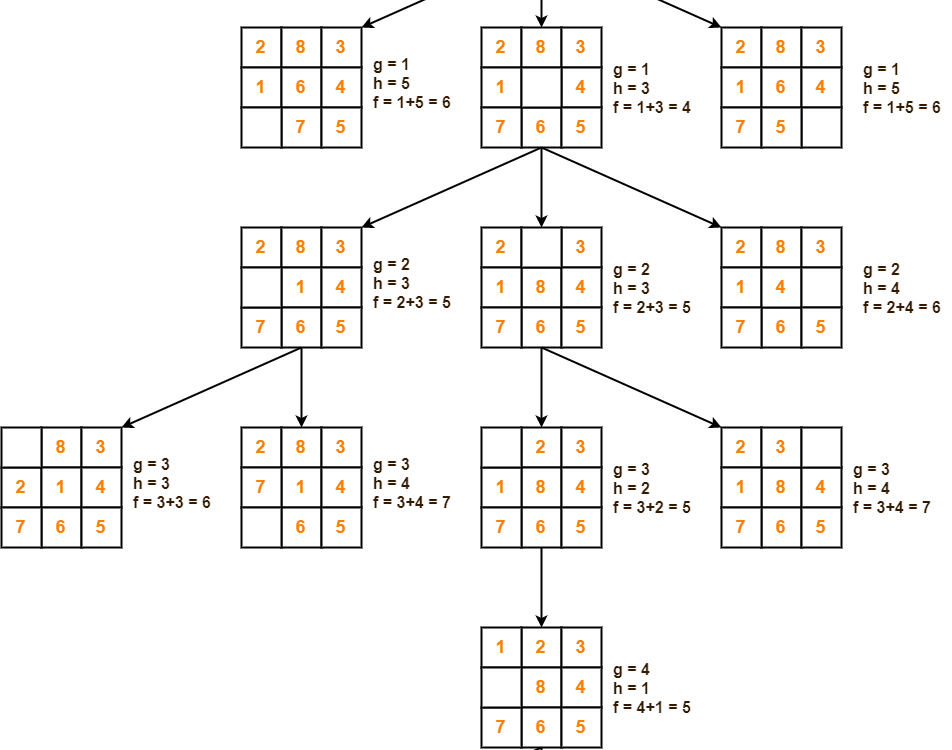
\includegraphics[keepaspectratio, width=0.75\linewidth]{images/Solve-Problem-01-05.png}
\end{center}
}

\only<7> {
\begin{center}
    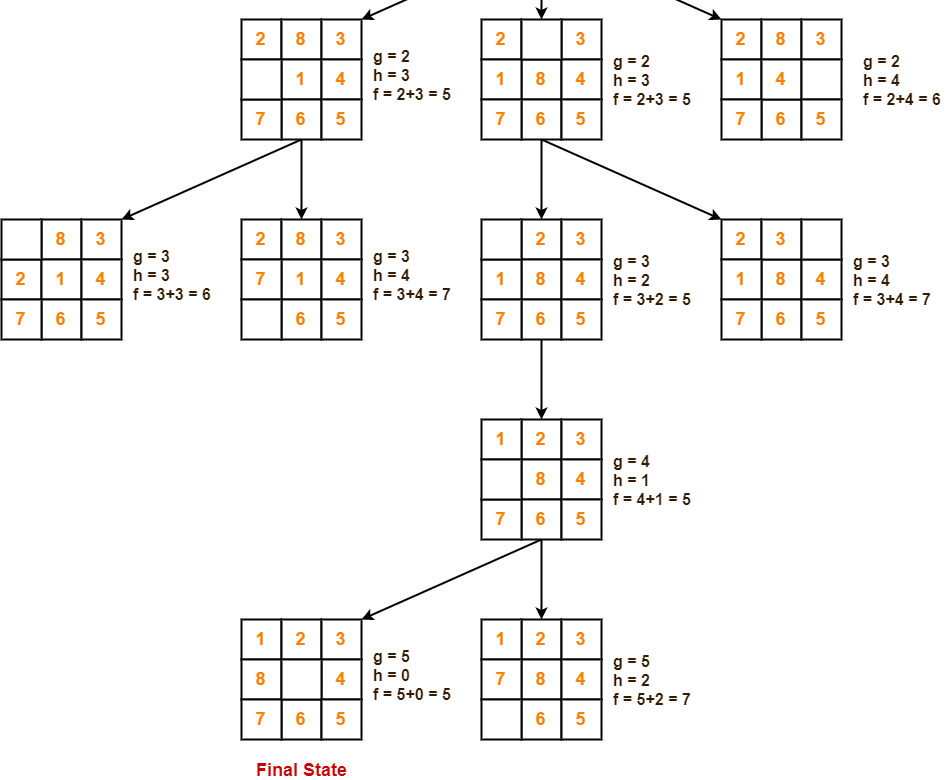
\includegraphics[keepaspectratio, width=0.75\linewidth]{images/Solve-Problem-01-06.png}
\end{center}
}

\end{small}
\end{frame}

\begin{frame}{A* Search example (graph problem)}
\begin{small}

\only<1> {
\begin{center}
    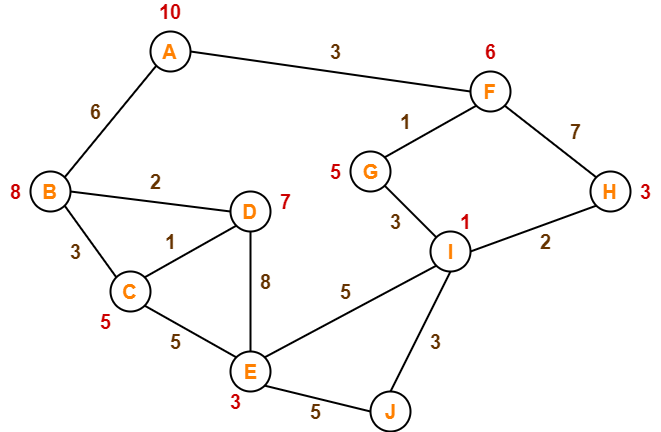
\includegraphics[keepaspectratio, width=0.60\linewidth]{images/A-Algorithm-Problem-02.png}
\end{center}

Find the most cost-effective path to reach from start state A to final state J using A* Algorithm.
}

\only<2> {
\begin{center}
    \vspace{-0.5cm}
    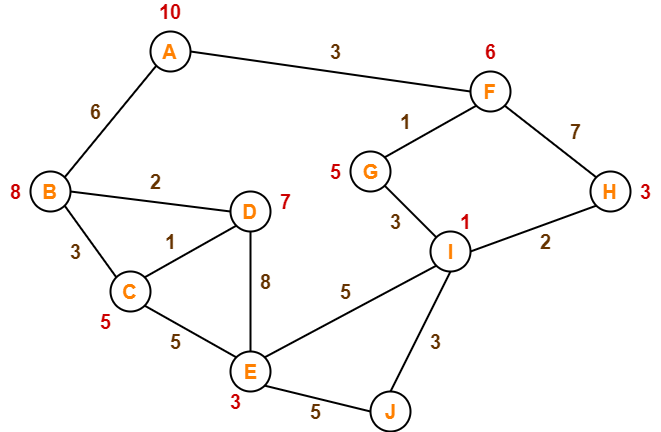
\includegraphics[keepaspectratio, width=0.40\linewidth]{images/A-Algorithm-Problem-02.png}
\end{center}

\vspace{-1cm}

\textbf{Step 1}:

We start with node A. Node B and Node F can be reached from node A.

A* Algorithm calculates $f(B)$ and $f(F)$:
\begin{itemize}
    \item $f(B) = 6 + 8 = 14$
    \item $f(F) = 3 + 6 = 9$
\end{itemize}

Since $f(F) < f(B)$, so it decides to go to node F.

Path: \textcolor{CS-1}{A $\rightarrow$ F}
}

\only<3> {
\begin{center}
    \vspace{-0.5cm}
    \includegraphics[keepaspectratio, width=0.40\linewidth]{images/A-Algorithm-Problem-02.png}
\end{center}

\vspace{-1cm}

\textbf{Step 2}:

Node G and Node H can be reached from node F.

A* Algorithm calculates $f(G)$ and $f(H)$.

\begin{itemize}
    \item $f(G) = (3+1) + 5 = 9$
    \item $f(H) = (3+7) + 3 = 13$
\end{itemize}

Since $f(G) < f(H)$, so it decides to go to node G.

Path: \textcolor{CS-1}{A $\rightarrow$ F $\rightarrow$ G}
}

\only<4> {
\begin{center}
    \vspace{-0.5cm}
    \includegraphics[keepaspectratio, width=0.40\linewidth]{images/A-Algorithm-Problem-02.png}
\end{center}

\vspace{-1cm}

\textbf{Step 3}:

Node I can be reached from node G.

A* Algorithm calculates $f(I)$.

\begin{itemize}
    \item $f(I) = (3+1+3) + 1 = 8$
\end{itemize}

It decides to go to node I.

Path: \textcolor{CS-1}{A $\rightarrow$ F $\rightarrow$ G $\rightarrow$ I}
}

\only<5> {
\begin{center}
    \vspace{-0.4cm}
    \includegraphics[keepaspectratio, width=0.40\linewidth]{images/A-Algorithm-Problem-02.png}
\end{center}

\vspace{-1cm}

\textbf{Step 4}:

Node E, Node H and Node J can be reached from node I.

A* Algorithm calculates $f(E)$, $f(H)$ and $f(J)$.

\begin{itemize}
    \item $f(E) = (3+1+3+5) + 3 = 15$
    \item $f(H) = (3+1+3+2) + 3 = 12$
    \item $f(J) = (3+1+3+3) + 0 = 10$
\end{itemize}
 
Since $f(J)$ is least, so it decides to go to node J.

Path: \textcolor{CS-1}{A $\rightarrow$ F $\rightarrow$ G $\rightarrow$ I $\rightarrow$ J}
}

\only<6> {
\begin{center}
    \includegraphics[keepaspectratio, width=0.75\linewidth]{images/A-Algorithm-Problem-02-Solution.png}
\end{center}
}

\end{small}
\end{frame}

\begin{frame}{Properties of A*}
\begin{small}

\begin{itemize}
    \item Optimal.
    \item Complete unless there are infinitely many nodes with $f \leq f(G)$.
    \item Keep all nodes in memory.
    \item A* search algorithm has some complexity issues.
\end{itemize}

\end{small}
\end{frame}

\begin{frame}{Local Search Methods}
\begin{small}

In many optimization problems, the state space is the space of all possible complete solutions:
\begin{itemize}
    \item We have an objective function that tells us how “good” a given state is, and we want to find the solution (goal) by minimizing or maximizing the value of this function.
    \item The start state may not be specified.
    \item The path to the goal doesn’t matter.
\end{itemize}

$\rightarrow$ In such cases, we can use \textcolor{CS-1}{local search algorithms} that keep a single “current” state and gradually try to improve it.

\end{small}
\end{frame}

\begin{frame}{Traveling Salesman problem example}
\begin{small}

Find the shortest tour connecting $n$ cities !

\begin{itemize}
    \item State space: All possible tours.
    \item Objective function: Length of tour.
\end{itemize}

What’s a possible local improvement strategy? Start with any complete tour, perform pairwise exchanges, ...

\begin{center}
    \includegraphics[keepaspectratio, width=0.75\linewidth]{images/salesman_problem.png}
\end{center}
\end{small}
\end{frame}

\begin{frame}{Hill climbing search}
\begin{small}

\textbf{Hill climbing algorithm} moves in the direction of increasing value to find the best solution. It terminates when it reaches a peak where no neighbor has a higher value.

\vspace{-2mm}
\textbf{function} \texttt{HillClimbing}(\emph{startNode}):\\

\begin{minipage}{0.10\linewidth}\vspace{0pt}%
\end{minipage}
\hskip10pt
\begin{minipage}{0.90\linewidth}\vspace{0pt}%	
\begin{algorithm}[H]
    currentNode = startNode\;
	\While{\emph{currentNode} \textbf{is not} \emph{null}}
 	{
  		neighborsNode = getNeighbors(currentNode)\;
        nextEval = -1\; 
        nextNode = \emph{null}\;
        \ForEach{$n$ node \textbf{in} neighborsNode}
  		{
            \If{getEval(n) > nextEval}
  		    {
                nextNode = n\;
                nextEval = getEval(n)\;
            }
  		}
        
  		\If{nextEval $\leq$ getEval(currentNode)}
  		{
  		    \textbf{return} currentNode\;
  		}
  		currentNode = nextNode\;
  	}
\end{algorithm}
\end{minipage}

\end{small}
\end{frame}

\begin{frame}{Hill climbing search}
\begin{small}

\begin{itemize}
    \item Not optimal and not complete.
    \item Can get stuck in local optima
    \item Variants: Choose first better successor, randomly choose among better successors,...
\end{itemize}

\begin{center}
    \includegraphics[keepaspectratio, width=0.75\linewidth]{images/local_optima.png}
\end{center}

\end{small}
\end{frame}

\subsection{Summary}

\begin{frame}{Classes of search}
\begin{small}

\textbf{Different classes of search} \cite{Russell2002}:

\begin{tabular}{l l l}
\textbf{Class} & \textbf{Name} & \textbf{Operation}\\
Any Path Uninformed & Depth-First & Systematic exploration of whole\\
                    & Breadth-First & tree until a goal nod is found\\
Any Path Informed & Best-First & Uses heuristic measure of goodness\\
                  &            & of a node\\
Optimal Uninformed & Uniform-Cost & Uses path "length" measure\\
Optimal Informed & A* & Uses path "length" measure and heuristic\\
\end{tabular}

\end{small}
\end{frame}

\begin{frame}{Informed vs Uninformed searches?}
\begin{small}

\textbf{Comparison between informed and uninformed searches} \cite{Russell2002}:

\begin{tabular}{l l l}
 & \textbf{Informed search} & \textbf{Uninformed search}\\
\textbf{Knowledge} & Uses knowledge & No use of knowledge (brute-force)\\
\textbf{Cost} & Low & Comparatively high\\
\textbf{Speed} & Fast & Slow\\
\textbf{Efficiency} & Hight (less time and cost) & Not so efficient\\
\end{tabular}

\end{small}
\end{frame}

\begin{frame}
\begin{center}
\textbf{\textcolor{CS-1light}{It's up to you !! You can do the third practical work.}}
\end{center}
\end{frame}

\begingroup
\setbeamertemplate{footline}{}
\appendix

\begin{frame}[allowframebreaks]{References}
	\tiny
	\bibliography{publications}
	\bibliographystyle{apalike}
\end{frame}
\endgroup

\end{document}
